\chapter[Produto Disponibilizado]{Produto Disponibilizado}
Esta seção procura apresentar o produto que foi disponibilizado após a aplicação de todas as correções e ajustes necessários para garantir o funcionamento do Agromart. Além disso, foram feitas atualizações de documentação nos arquivos README.md dos reposítórios do aplicativo e da API principal. Essas atualizações foram realizadas para oferecer uma visão mais clara do funcionamento do Agromart, facilitando o entendimento e a utilização por parte dos usuários. Além disso também ajuda na compreensão dos futuros desenvolvedores colaboradores, de modo que podem conseguir rapidamente entender as funcionalidades do sistema. 

\section{Funcionalidades do Painel da CSA}
O conteúdo de cada CSA é armazenado em um CMS (Sistema de Gerenciamento de Conteúdo), que possui um painel que possibilita que os administradores de uma CSA insiram as informações das loja e dos seus produtos, além de possibilitar visualizar as informações de cada consumidor. Após o trabalho realizado, as seguinte funcionalidades estão disponíveis no MVP para serem utilizadas através do Painel de Gerenciamento da CSA:

\begin{itemize}
    \item Gerenciamento de loja
    \item Gerenciamento de produtos avulso
    \item Gerenciamento de cestas
    \item Gerenciamento de planos
    \item Gerenciamento de assinaturas
    \item Gerenciamento de usuários
    \item Gerenciamento de endereços
    \item Gerenciamento de pedidos
\end{itemize}

\subsection{Gerenciar Lojas}
Na tela de gerenciamento de loja indicada na Figura \ref{tela-lojas-cms}, é possível ver as lojas já cadastradas pela sua CSA, também é possível criar uma nova loja, editar uma loja já existe e deletar uma loja.

\begin{figure}[h]
	\centering
	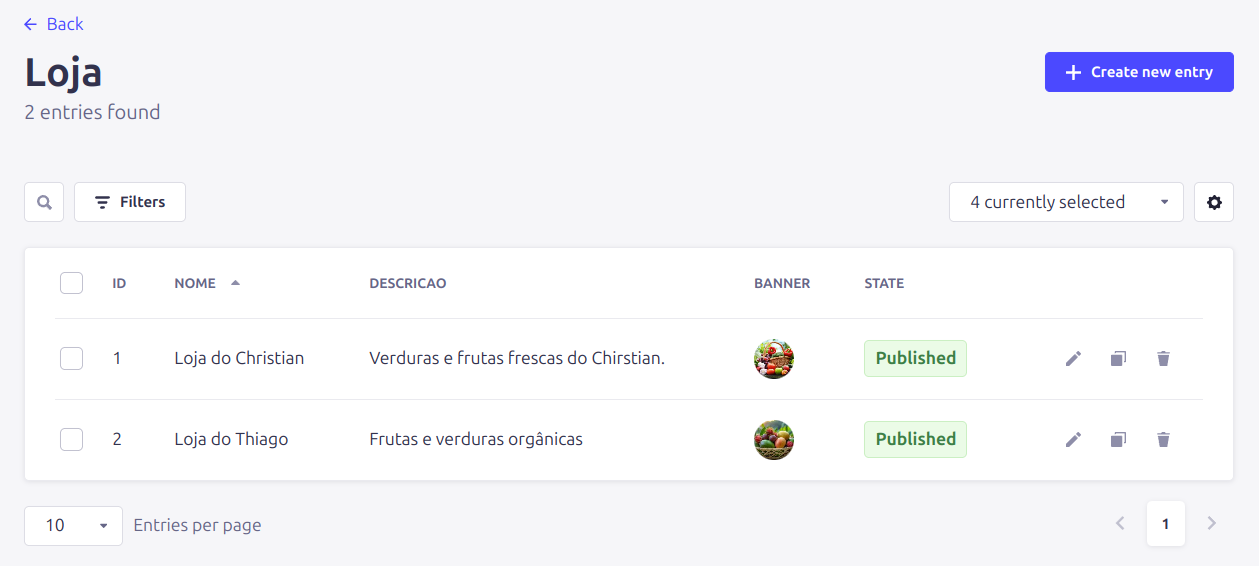
\includegraphics[keepaspectratio=true,scale=0.28]{figuras/painel_lojas.png}
	\caption{Tela de lojas da CSA}
        \label{tela-lojas-cms}
\end{figure}

\subsection{Gerenciar Cestas}
Na tela de gerenciamento de loja indicada na Figura \ref{tela-cestas-cms}, é possível ver as cestas já cadastradas pela sua CSA, também é possível criar uma nova cesta, editar uma cesta já existe e deletar uma cesta.

\begin{figure}[h]
	\centering
	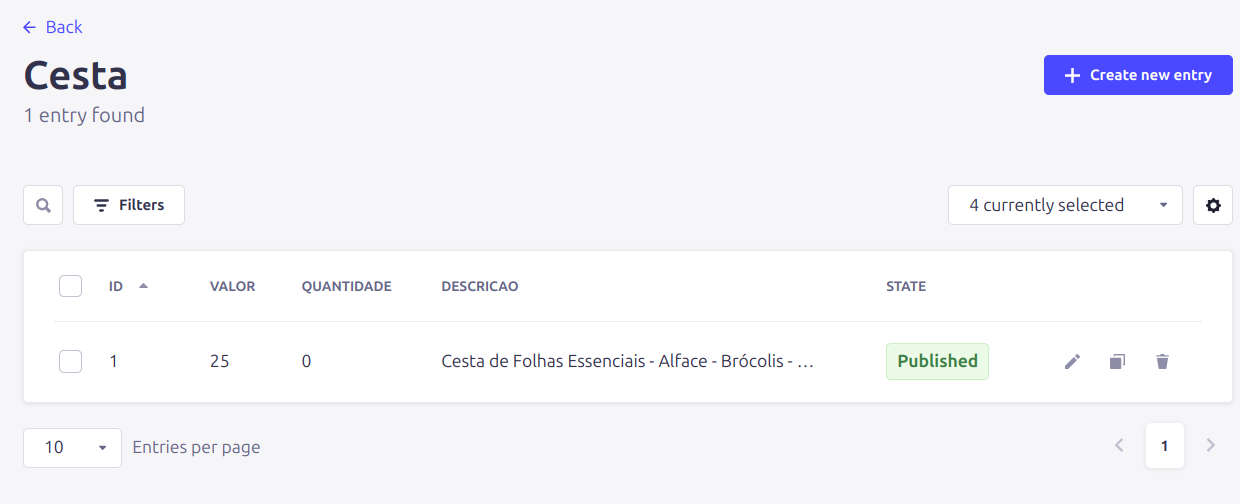
\includegraphics[keepaspectratio=true,scale=0.28]{figuras/painel_cestas.png}
	\caption{Tela de cestas}
        \label{tela-cestas-cms}
\end{figure}

\subsection{Gerenciar Planos}
Na tela de gerenciamento de planos indicada na Figura \ref{tela-planos-cms}, é possível ver os planos já cadastradas pela sua CSA, também é possível criar um novo plano, editar um plano já existe e deletar plano.

\begin{figure}[h]
	\centering
	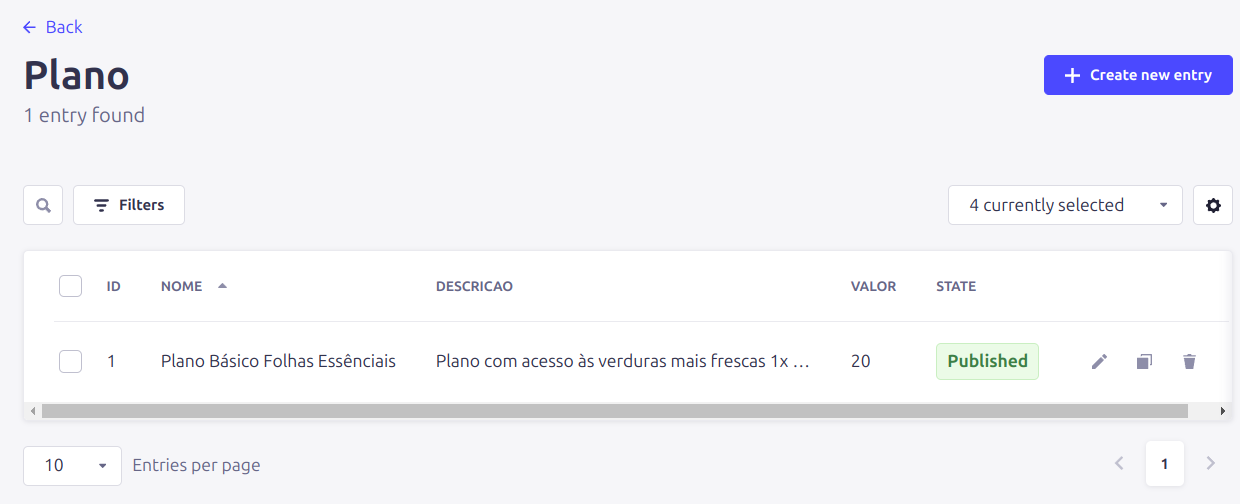
\includegraphics[keepaspectratio=true,scale=0.28]{figuras/painel_planos.png}
	\caption{Tela de planos}
        \label{tela-planos-cms}
\end{figure}

\subsection{Gerenciar Produtos Avulso}
Na tela de gerenciamento de produtos indicada na Figura \ref{tela-produtos-cms}, é possível ver os produtos avulsos já cadastradas pela sua CSA, também é possível criar novos produtos avulsos, editar um produto já existe e deletar um produto.

\begin{figure}[h]
	\centering
	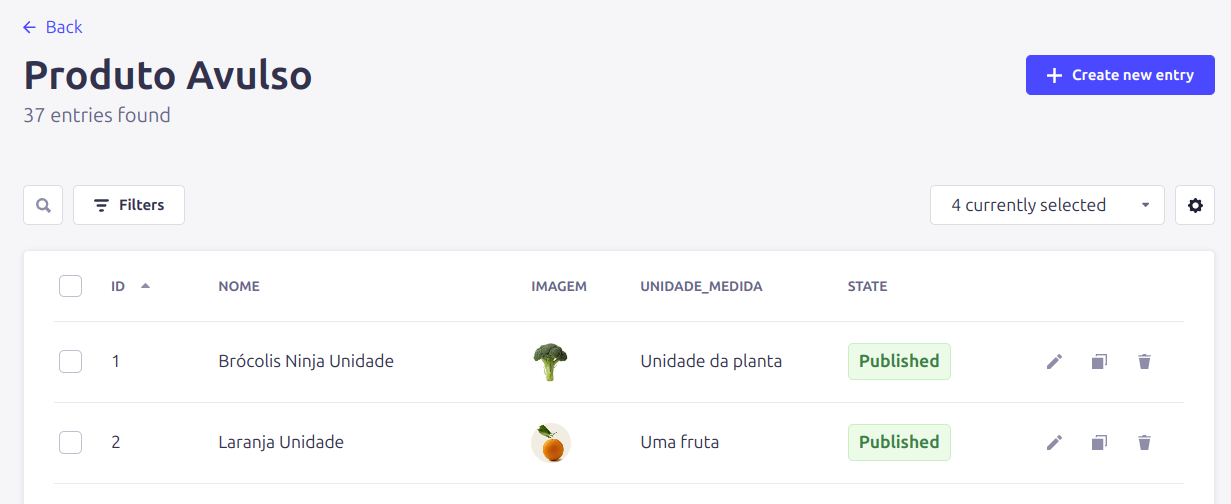
\includegraphics[keepaspectratio=true,scale=0.28]{figuras/painel_produtos.png}
	\caption{Tela de produtos avulsos}
        \label{tela-produtos-cms}
\end{figure}

\subsection{Gerenciar Assinaturas}
Na tela de gerenciamento de assinantes indicada na Figura \ref{tela-assinaturas-cms}, é possível visualizar quais são os assinantes de cada plano da CSA, além de possibilitar ao administrador saber quais assinantes desejam pular o recebimento da cesta semanal através do campo "pular\_cesta".

\begin{figure}[h]
	\centering
	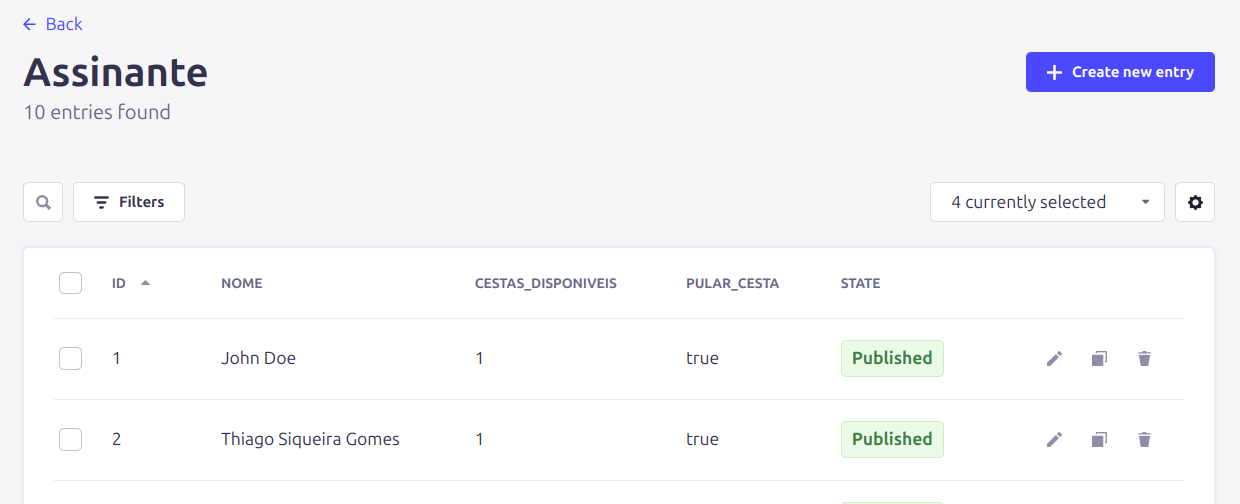
\includegraphics[keepaspectratio=true,scale=0.28]{figuras/painel_assinantes.png}
	\caption{Tela de assinaturas}
        \label{tela-assinaturas-cms}
\end{figure}

\subsection{Gerenciar Pedidos}
Na tela de gerenciamento de extrato mostrada na Figura \ref{tela-produtos-cms}, é possível verificar os pedidos realizados por cada usuário, além disso, nesta tela também é possível marcar cada pedido com dois status diferentes, o status "pagamento\_realizado" e o status "entregue", para que o administrador da CSA tenha controle da situação de cada pedido.

\begin{figure}[h]
	\centering
	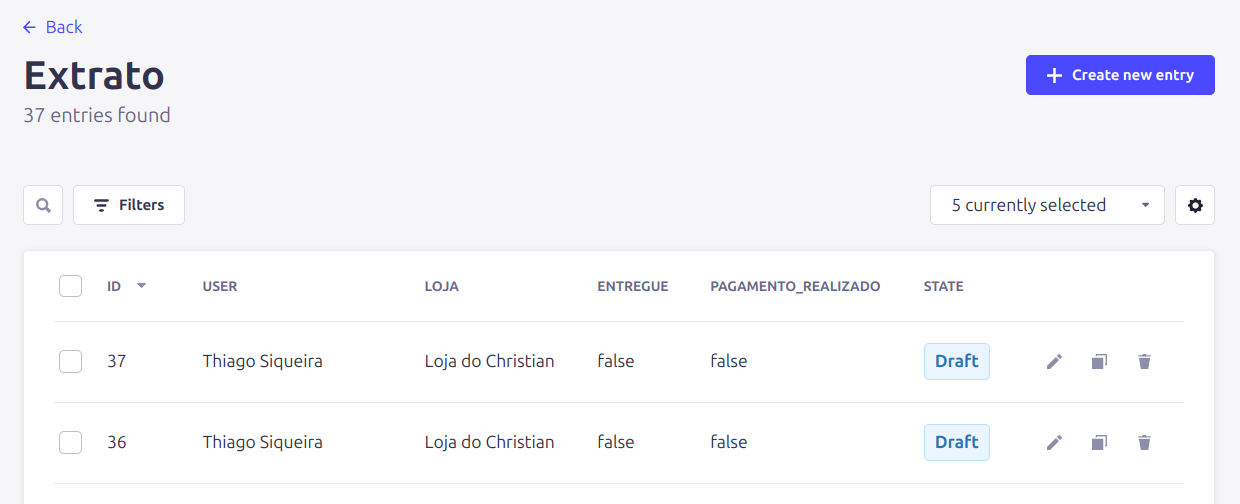
\includegraphics[keepaspectratio=true,scale=0.28]{figuras/painel_extrato.png}
	\caption{Tela de pedidos}
        \label{tela-peddos-cms}
\end{figure}

\subsection{Gerenciar Usuários}
Na tela de gerenciamento de usuários mostrada na Figura \ref{tela-usuarios-cms}, é possível ver informações de um usuário, nesta tela também é possível criar, excluir e editar um usuário se necessário.

\begin{figure}[h]
	\centering
	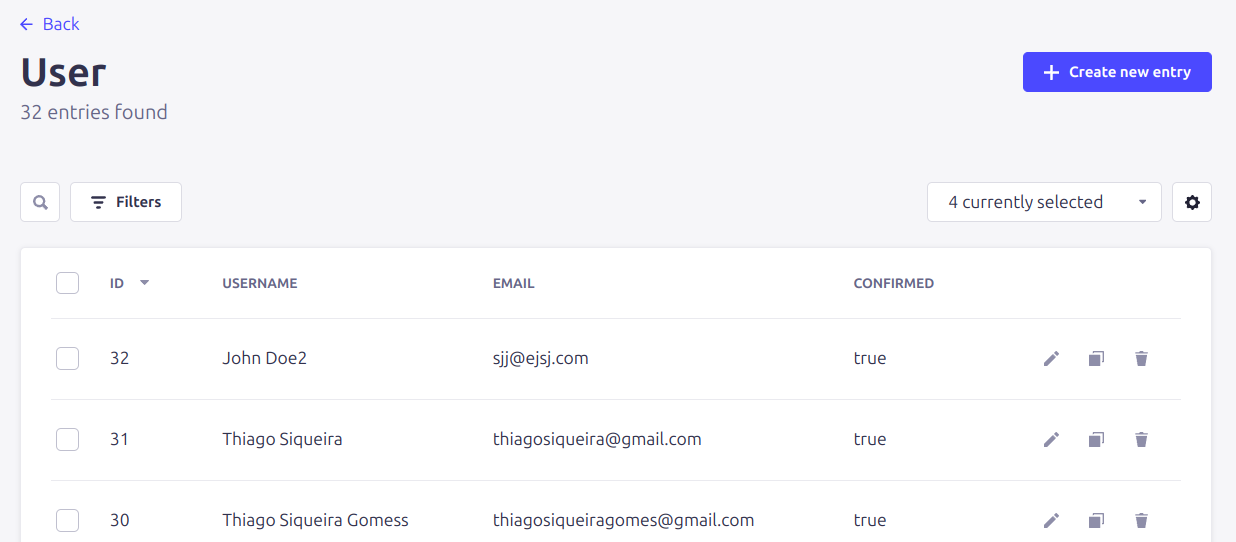
\includegraphics[keepaspectratio=true,scale=0.28]{figuras/painel_usuarios.png}
	\caption{Tela de usuários}
        \label{tela-usuarios-cms}
\end{figure}

\subsection{Gerenciar Endereços}
Na tela de gerenciamento de endereços mostrada na Figura \ref{tela-endereco-cms}, é possível verificar o endereço de um usuário, nesta tela também é possível criar, excluir e editar o endereço de um usuário se necessário.

\begin{figure}[h]
	\centering
	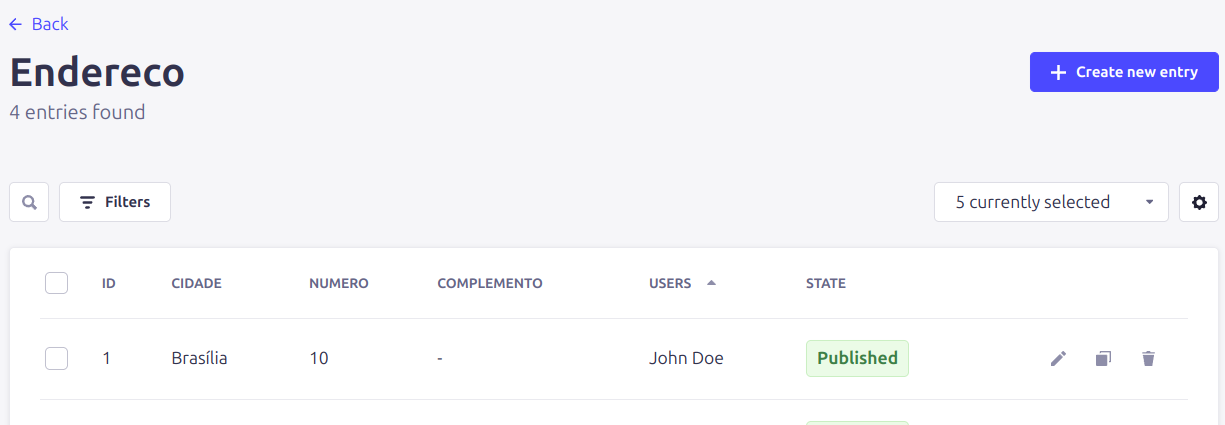
\includegraphics[keepaspectratio=true,scale=0.28]{figuras/painel_endereco.png}
	\caption{Tela de endereço}
        \label{tela-endereco-cms}
\end{figure}

\section{Funcionalidades do Aplicativo}
Após todas as correções realizadas para garantir o funcionamento do MVP do aplicativo móvel do Agromart, as seguintes funcionalidades estão disponíveis para uso:

\begin{itemize}
    \item Se conectar a uma CSA
    \item Visualização de todas as lojas de uma CSA na página principal
    \item Pesquisar lojas por nome
    \item Pesquisar lojas por região administrativa
    \item Visualização de loja com produtos, planos e cestas
    \item Link para contato com o dono da loja
    \item Realizar pedidos
    \item Visualizar histórico de pedidos
    \item Visualizar planos assinados e pular cesta da semana
    \item Cadastrar e editar endereço
    \item Editar perfil
\end{itemize}

\subsection{Se Conectar a uma CSA}
Na tela inicial mostrada na Figura \ref{tela-inicial-app}, utilizando o botão "Escolha sua CSA", o usuário será redirecionado para uma tela em que é possível digitar o código de uma CSA e pesquisar por ela, como mostrado na Figura \ref{tela-busca-csa-app}.

Ao encontrar a CSA desejada, é possível se conectar a essa CSA utilizando o botão "Utilizar esta CSA", como se pode ver na Figura \ref{tela-escolhe-csa-app}. Após se conectar à uma CSA, o usuário será redirecionado para tela de login e registro.

\begin{figure}[h]
	\centering
	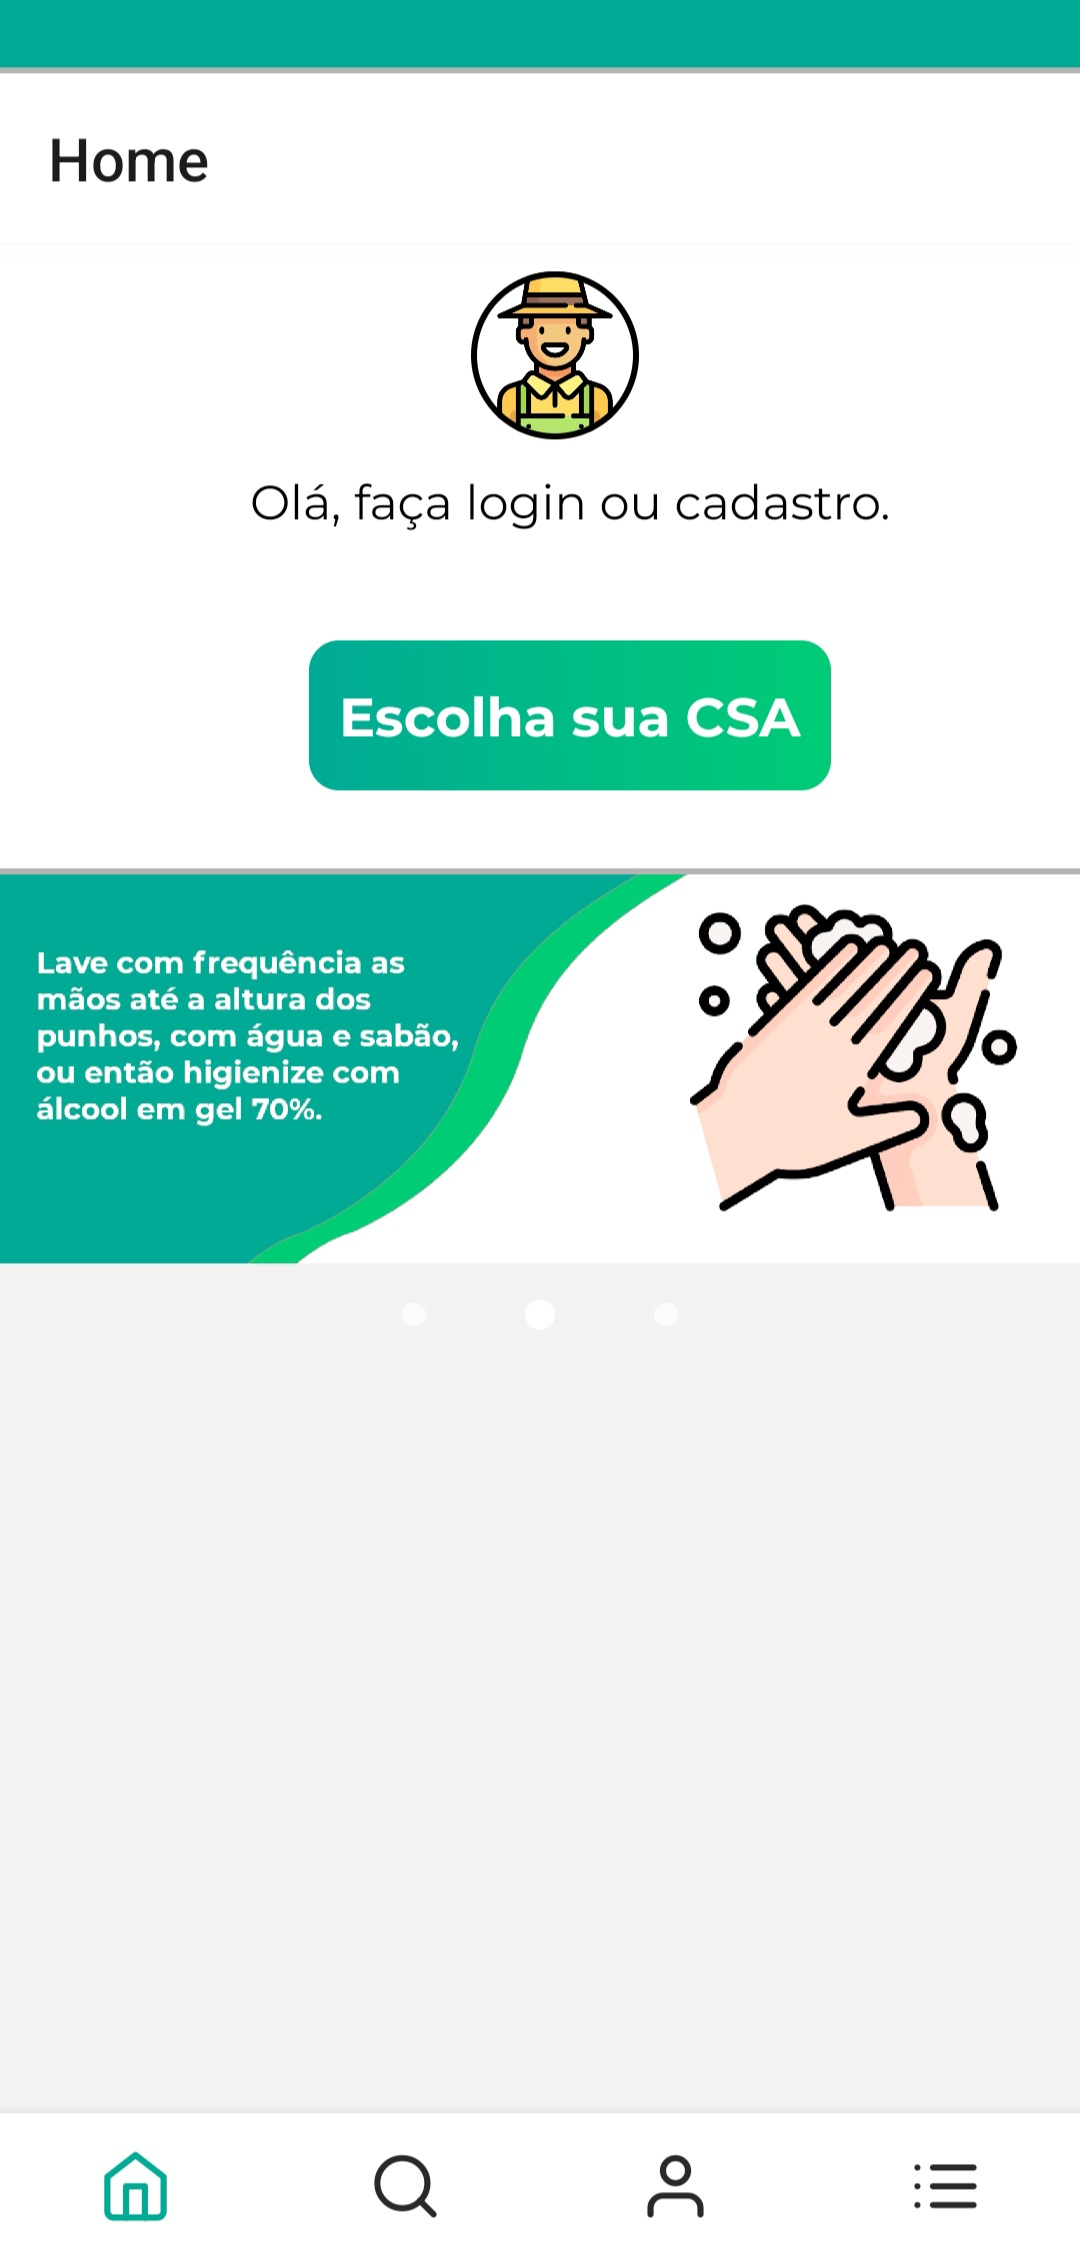
\includegraphics[keepaspectratio=true,scale=0.16]{figuras/inicial.jpg}
	\caption{Tela Inicial}
        \label{tela-inicial-app}
\end{figure}

\begin{figure}[h]
	\centering
	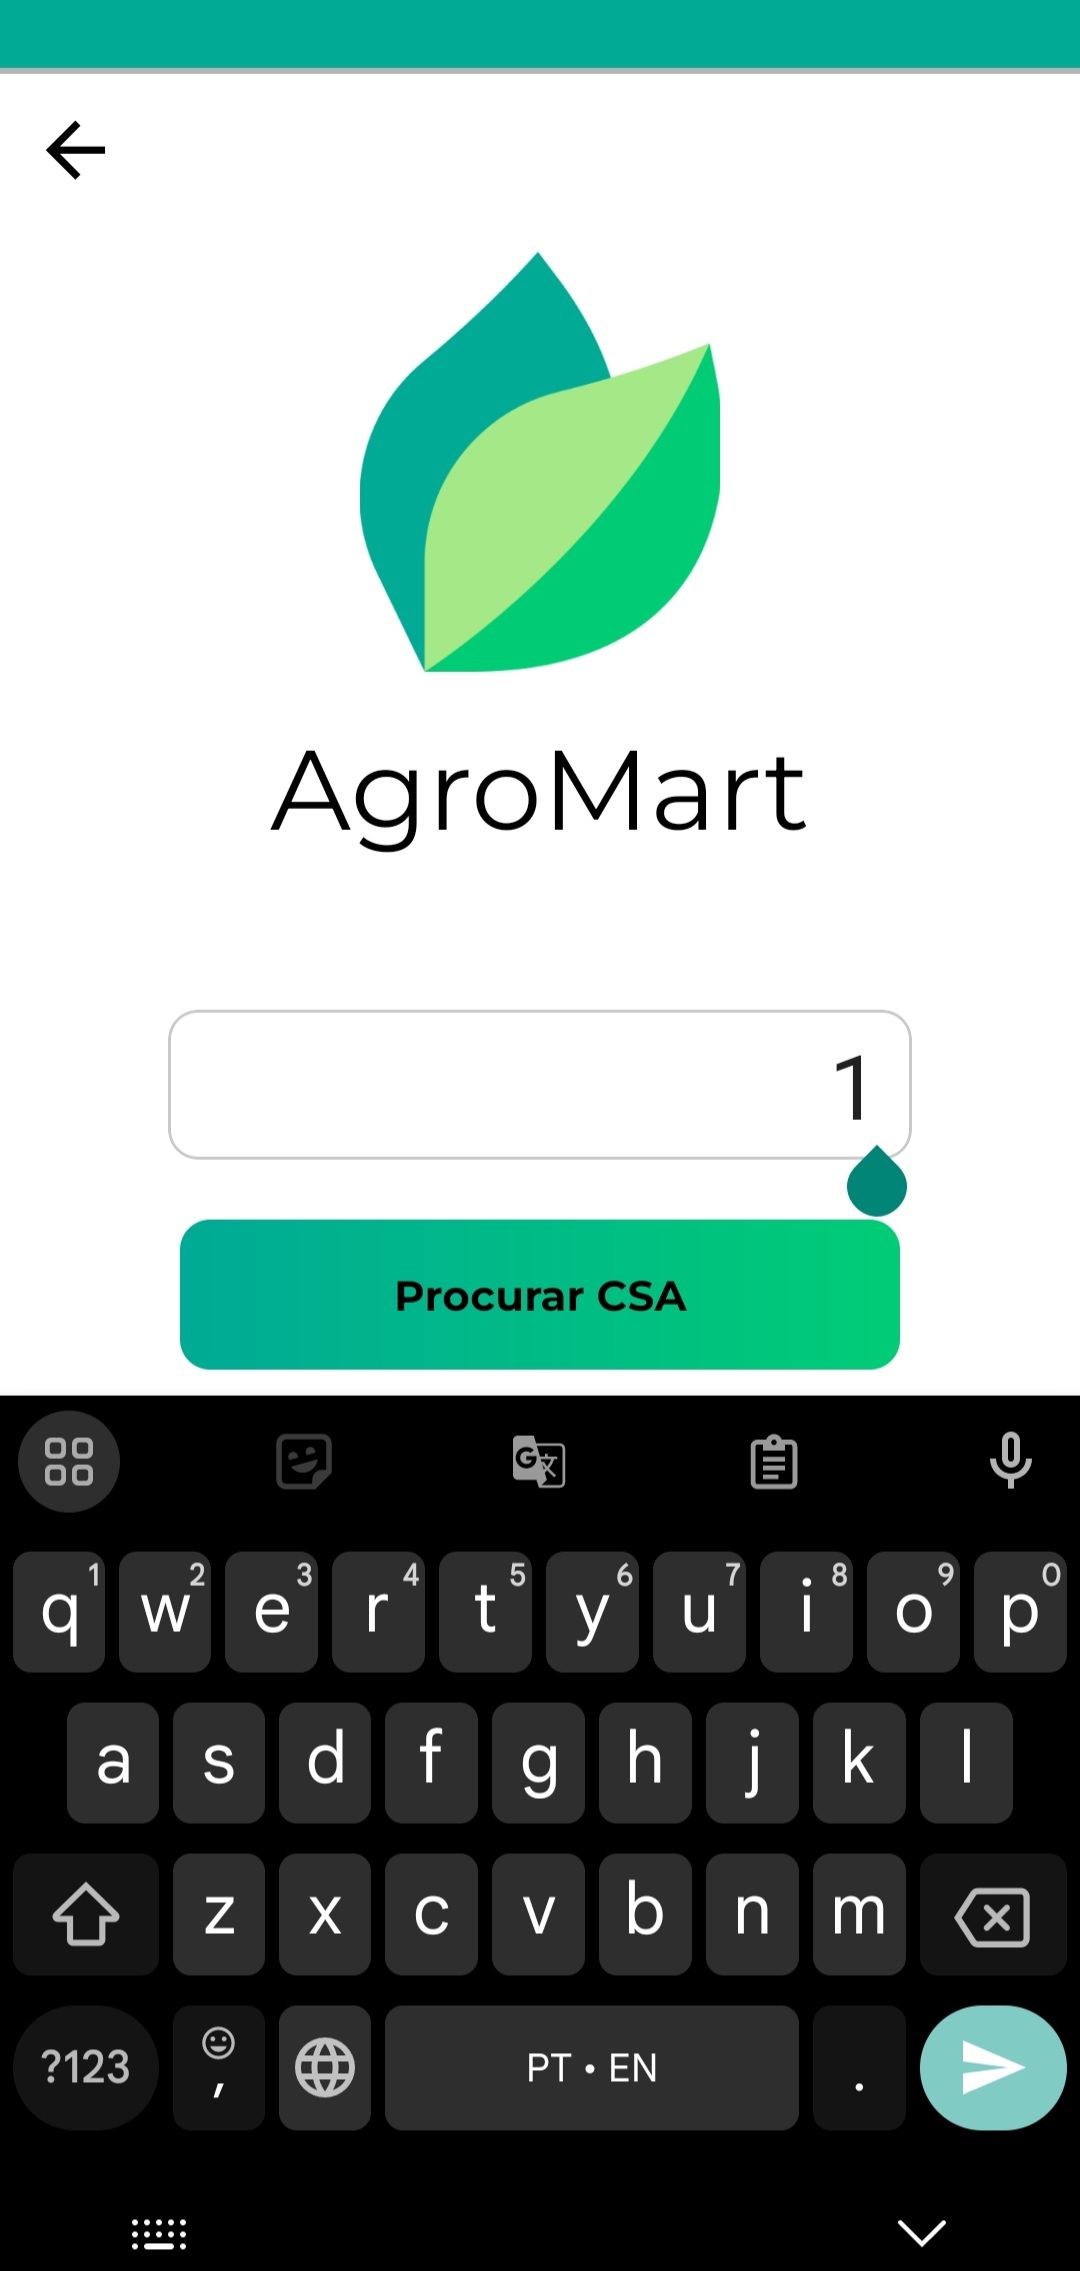
\includegraphics[keepaspectratio=true,scale=0.16]{figuras/pesquisa_csa.jpg}
	\caption{Tela de Busca de CSA}
        \label{tela-busca-csa-app}
\end{figure}

\begin{figure}[h]
	\centering
	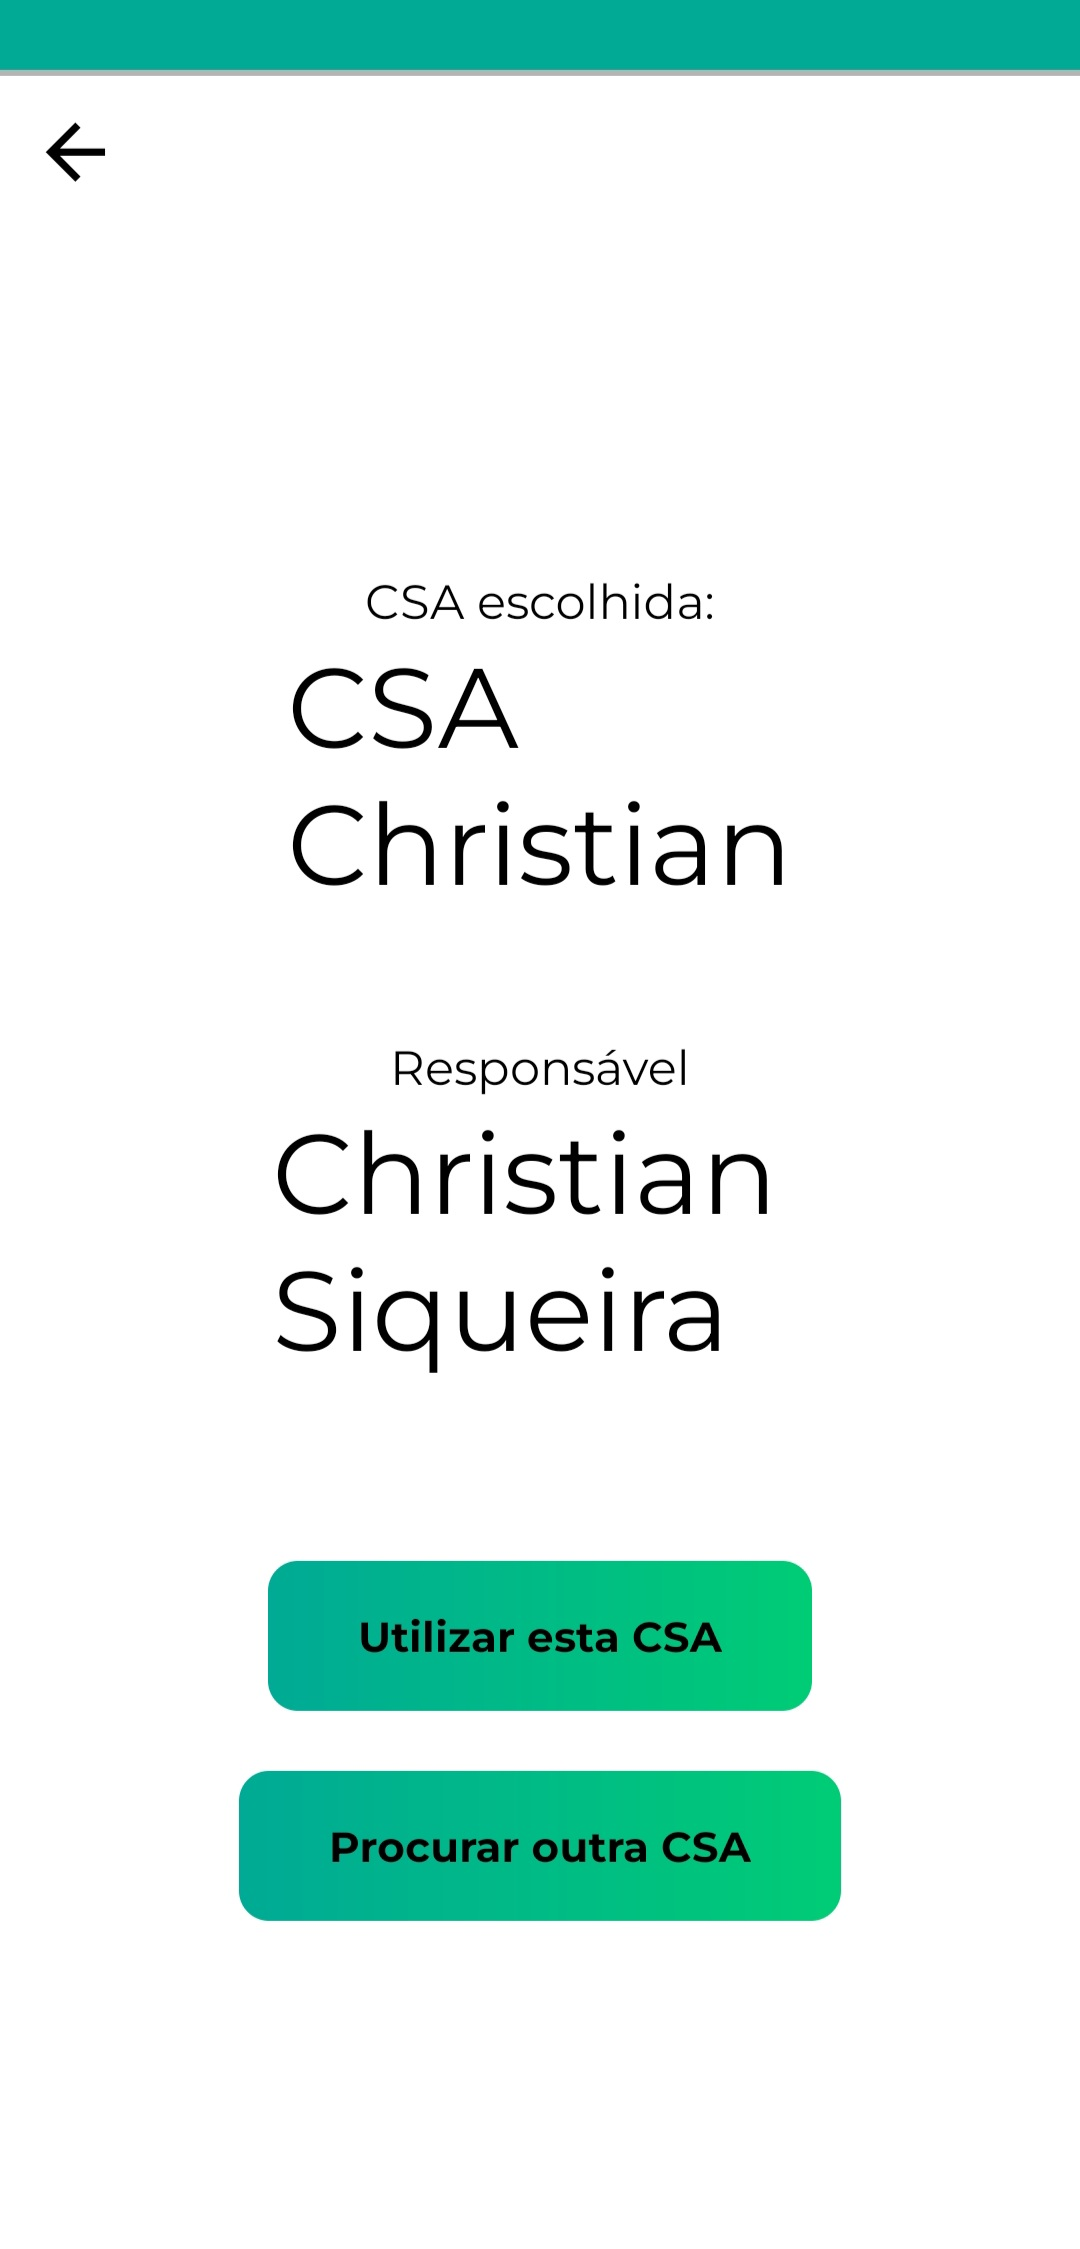
\includegraphics[keepaspectratio=true,scale=0.16]{figuras/seleciona_csa.jpg}
	\caption{Tela de Escolha de CSA}
        \label{tela-escolhe-csa-app}
\end{figure}

\subsection{Criar Conta na CSA}
Após escolher a CSA desejada, caso ainda não tenha um cadastro de usuário nesta CSA, é possível realizar o cadastro do seu perfil utilizando: nome, email e senha.

Na tela de criação de conta, mostrada na Figura \ref{tela-signup-csa-app}, é possível cadastrar seu perfil na CSA escolhida. O cadastro é realizado dentro do servidor de cada CSA individualmente, então as credenciais cadastradas poderão ser usadas apenas para realizar o acesso à CSA cadastrada.

\begin{figure}[h]
	\centering
	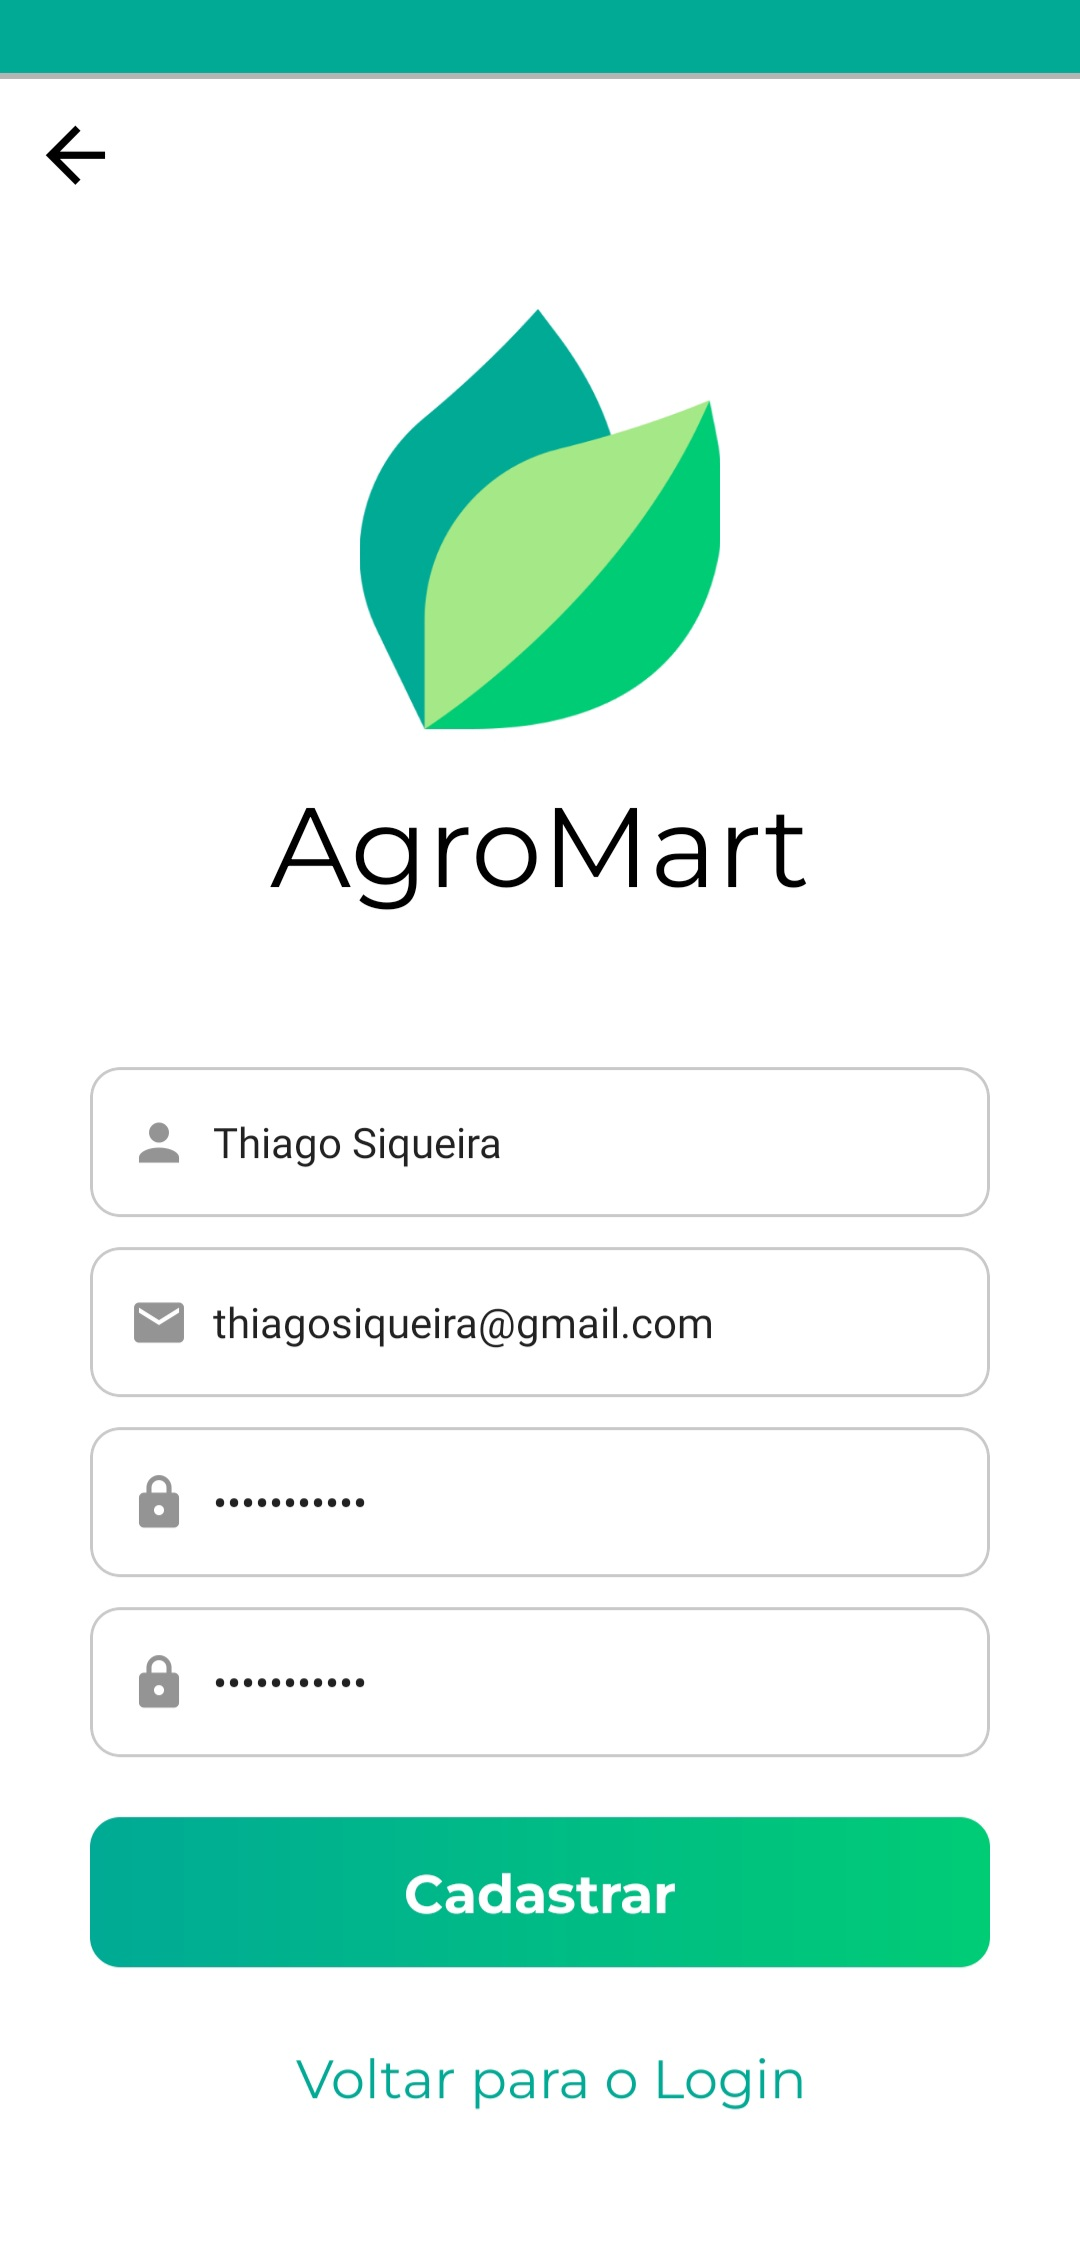
\includegraphics[keepaspectratio=true,scale=0.16]{figuras/signup_app.jpg}
	\caption{Tela de cadastro de usuário}
        \label{tela-signup-csa-app}
\end{figure}

\subsection{Login na CSA}
Após escolher a CSA desejada, caso já tenha um cadastro de usuário nesta CSA, é possível realizar o login no seu perfil utilizando email e senha, como mostra a Figura \ref{tela-login-csa-app}.

Nesta tela de Login também é possível conferir o nome e o domínio da CSA em que está se realizando login.

\begin{figure}[h]
	\centering
	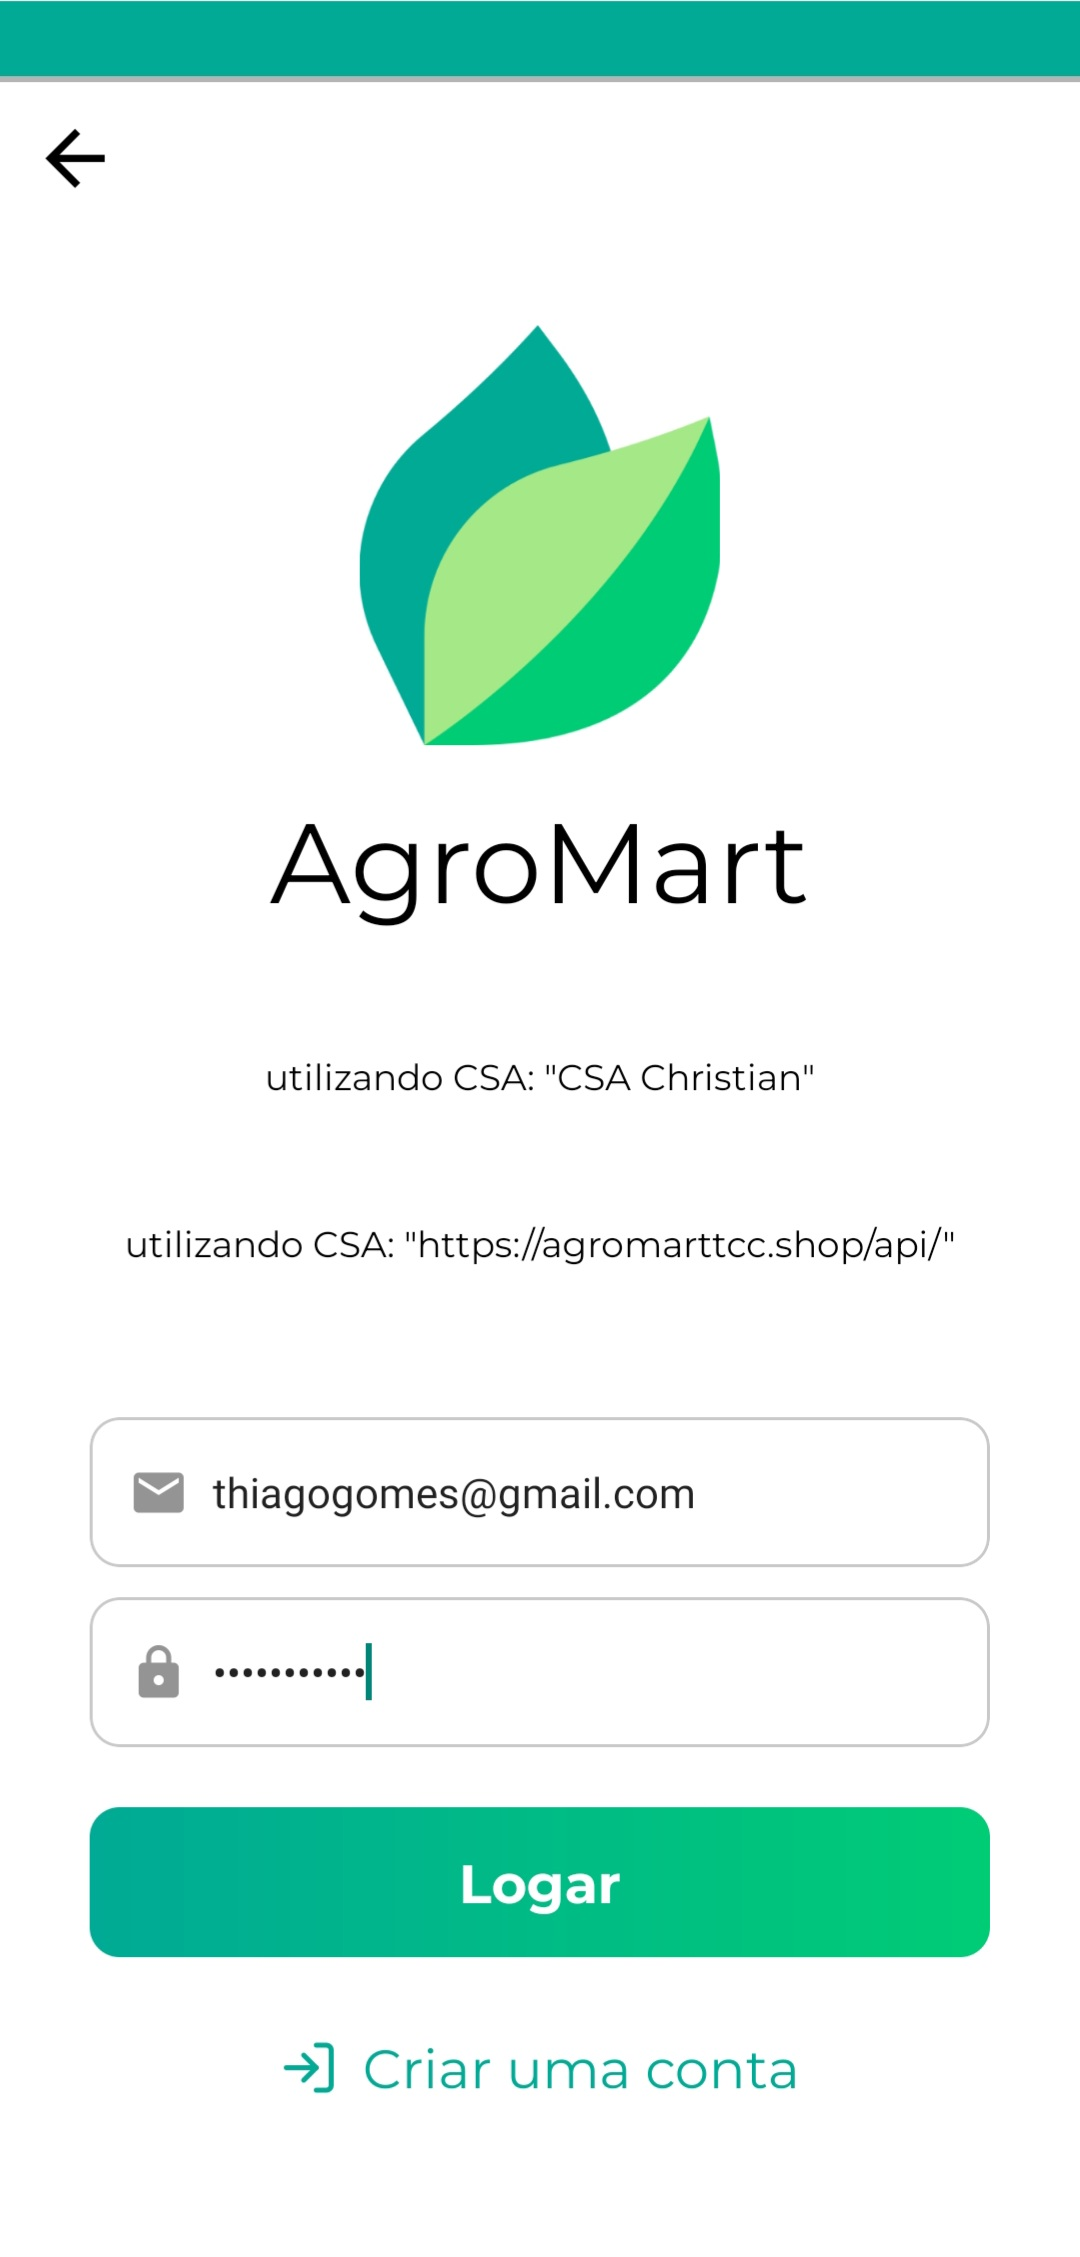
\includegraphics[keepaspectratio=true,scale=0.16]          {figuras/login_app.jpg}
	\caption{Tela de login de usuário}
        \label{tela-login-csa-app}
\end{figure}

\subsection{Visualizar Lojas na Página Principal}
Uma CSA pode ter várias lojas diferentes. Na página principal, mostrada na Figura \ref{tela-principal-loja-app}, é possível visualizar uma lista das lojas que esta CSA possui, como mostrado na Figura XX.

\begin{figure}[h]
	\centering
	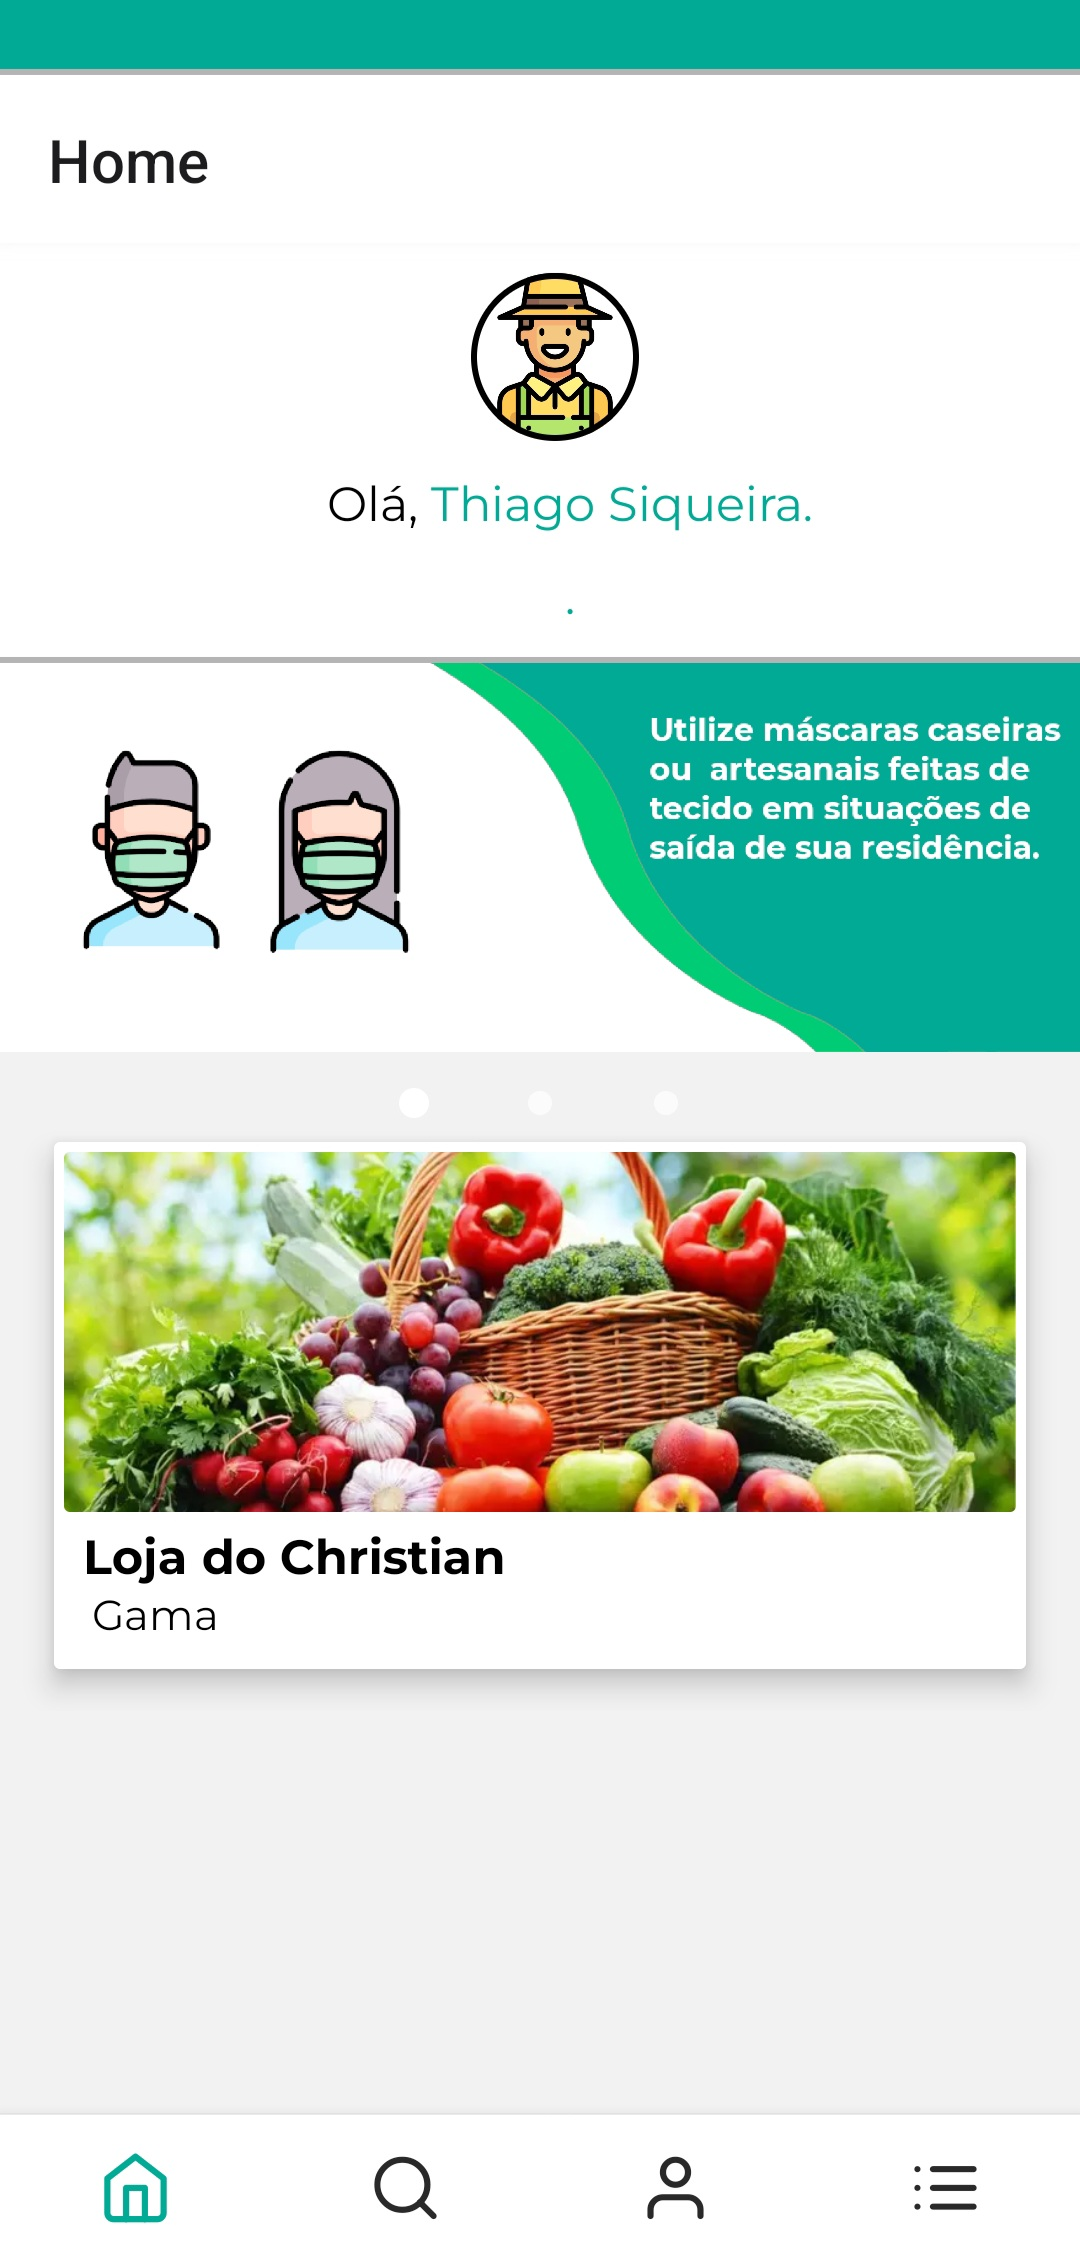
\includegraphics[keepaspectratio=true,scale=0.16]{figuras/principal.jpg}
	\caption{Página Principal}]
        \label{tela-principal-loja-app}
\end{figure}

\subsection{Pesquisar Loja por Nome}
Clicando no ícone em formato de lupa e digitando no campo de pesquisa, é possível pesquisar uma loja pelo nome ou por parte do nome, como mostra a Figura \ref{tela-pesquisa-loja-nome-app}.

\begin{figure}[h]
	\centering
	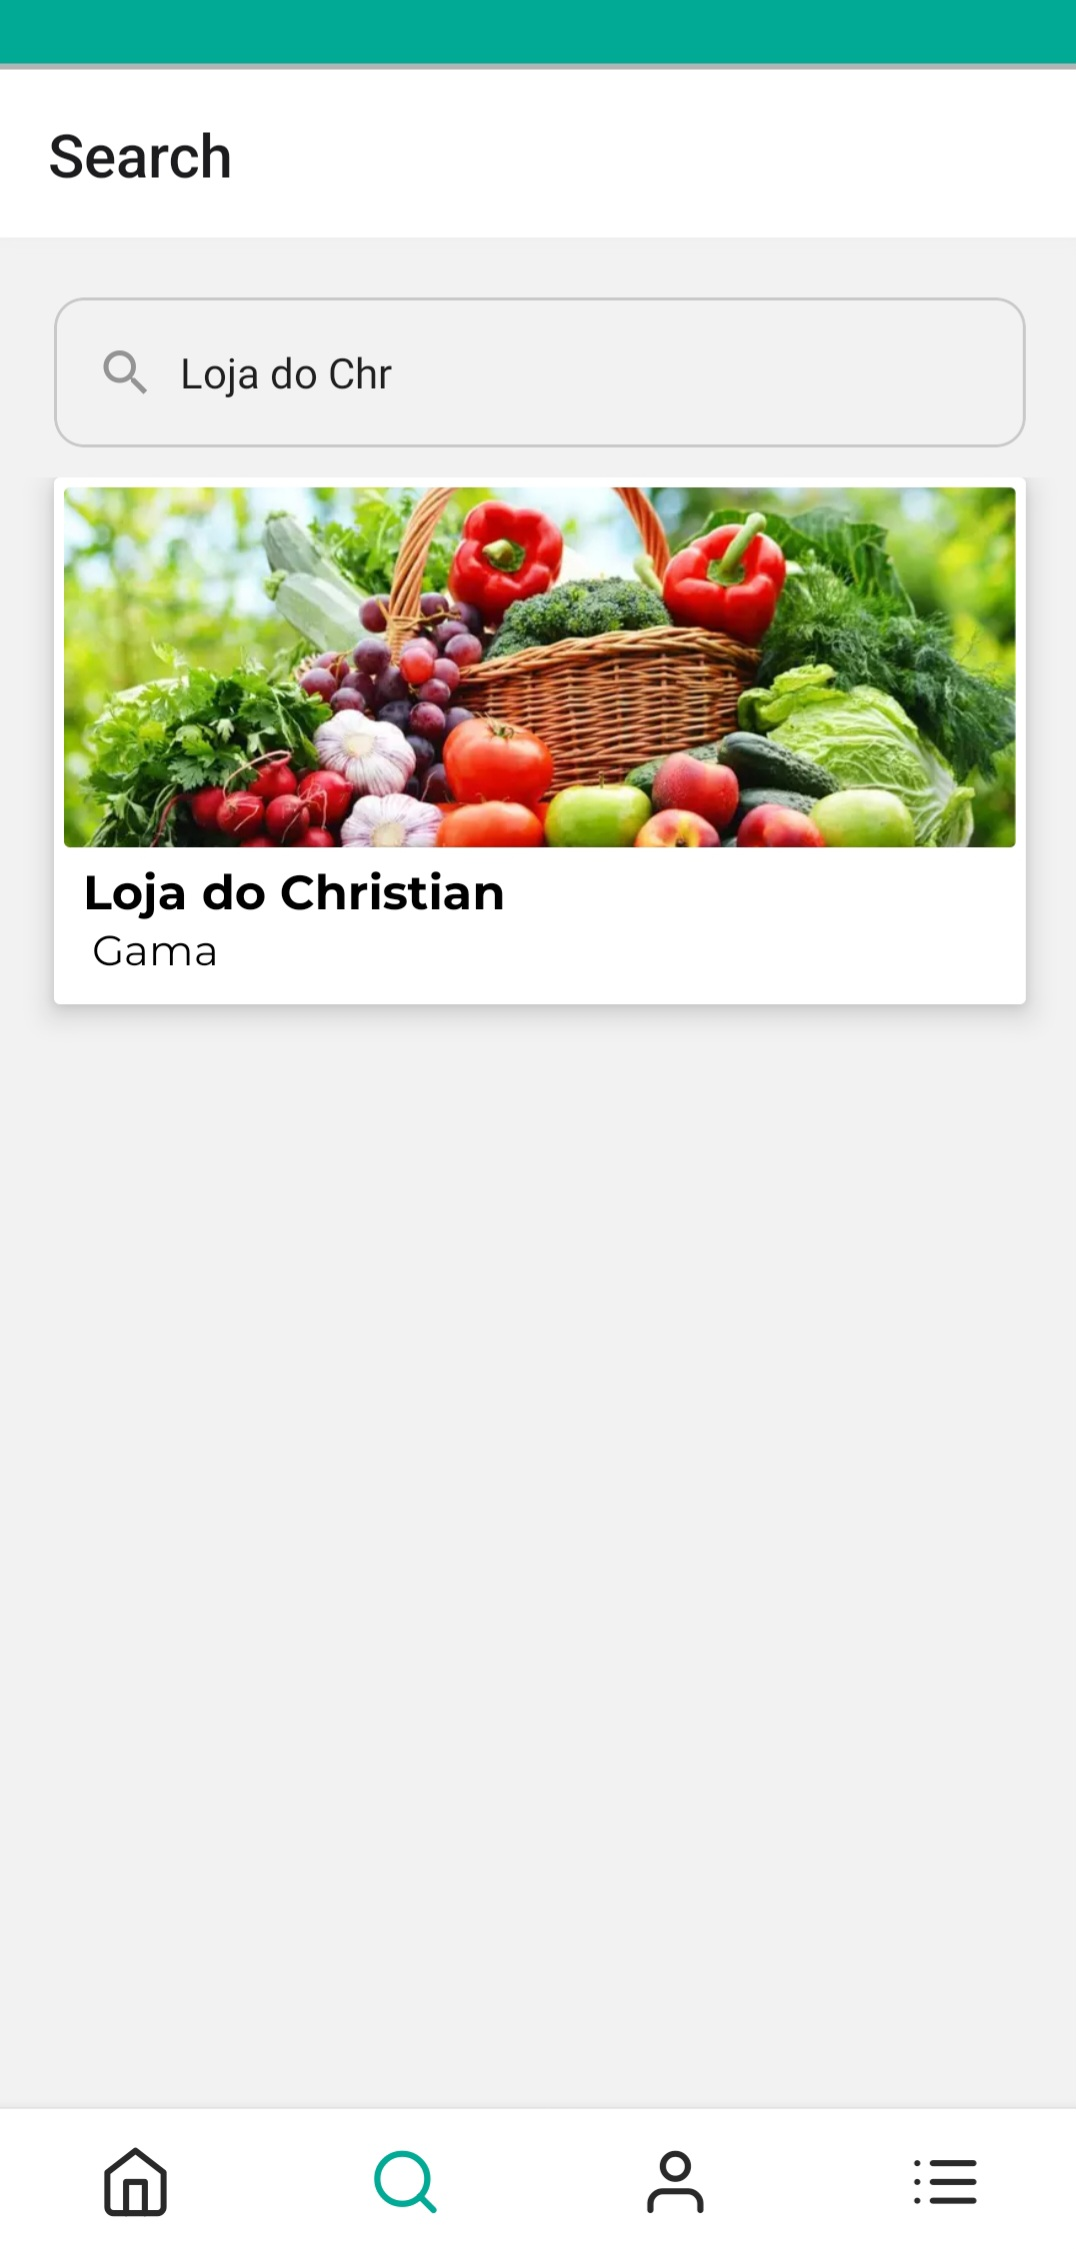
\includegraphics[keepaspectratio=true,scale=0.16]{figuras/filtra_loja_nome.jpg}
	\caption{Tela de pesquisa de loja por nome}
        \label{tela-pesquisa-loja-nome-app}
\end{figure}

\subsection{Pesquisar Loja por Região Administrativa}
Na tela mostrada na Figura \ref{tela-pesquisa-loja-regiao-app}, é possível visualizar todas as regiões administrativas do Distrito Federal, clicando na região administrativa desejada é possível ver uma lista de todas as lojas disponíveis nesta região.

\begin{figure}[h]
	\centering
	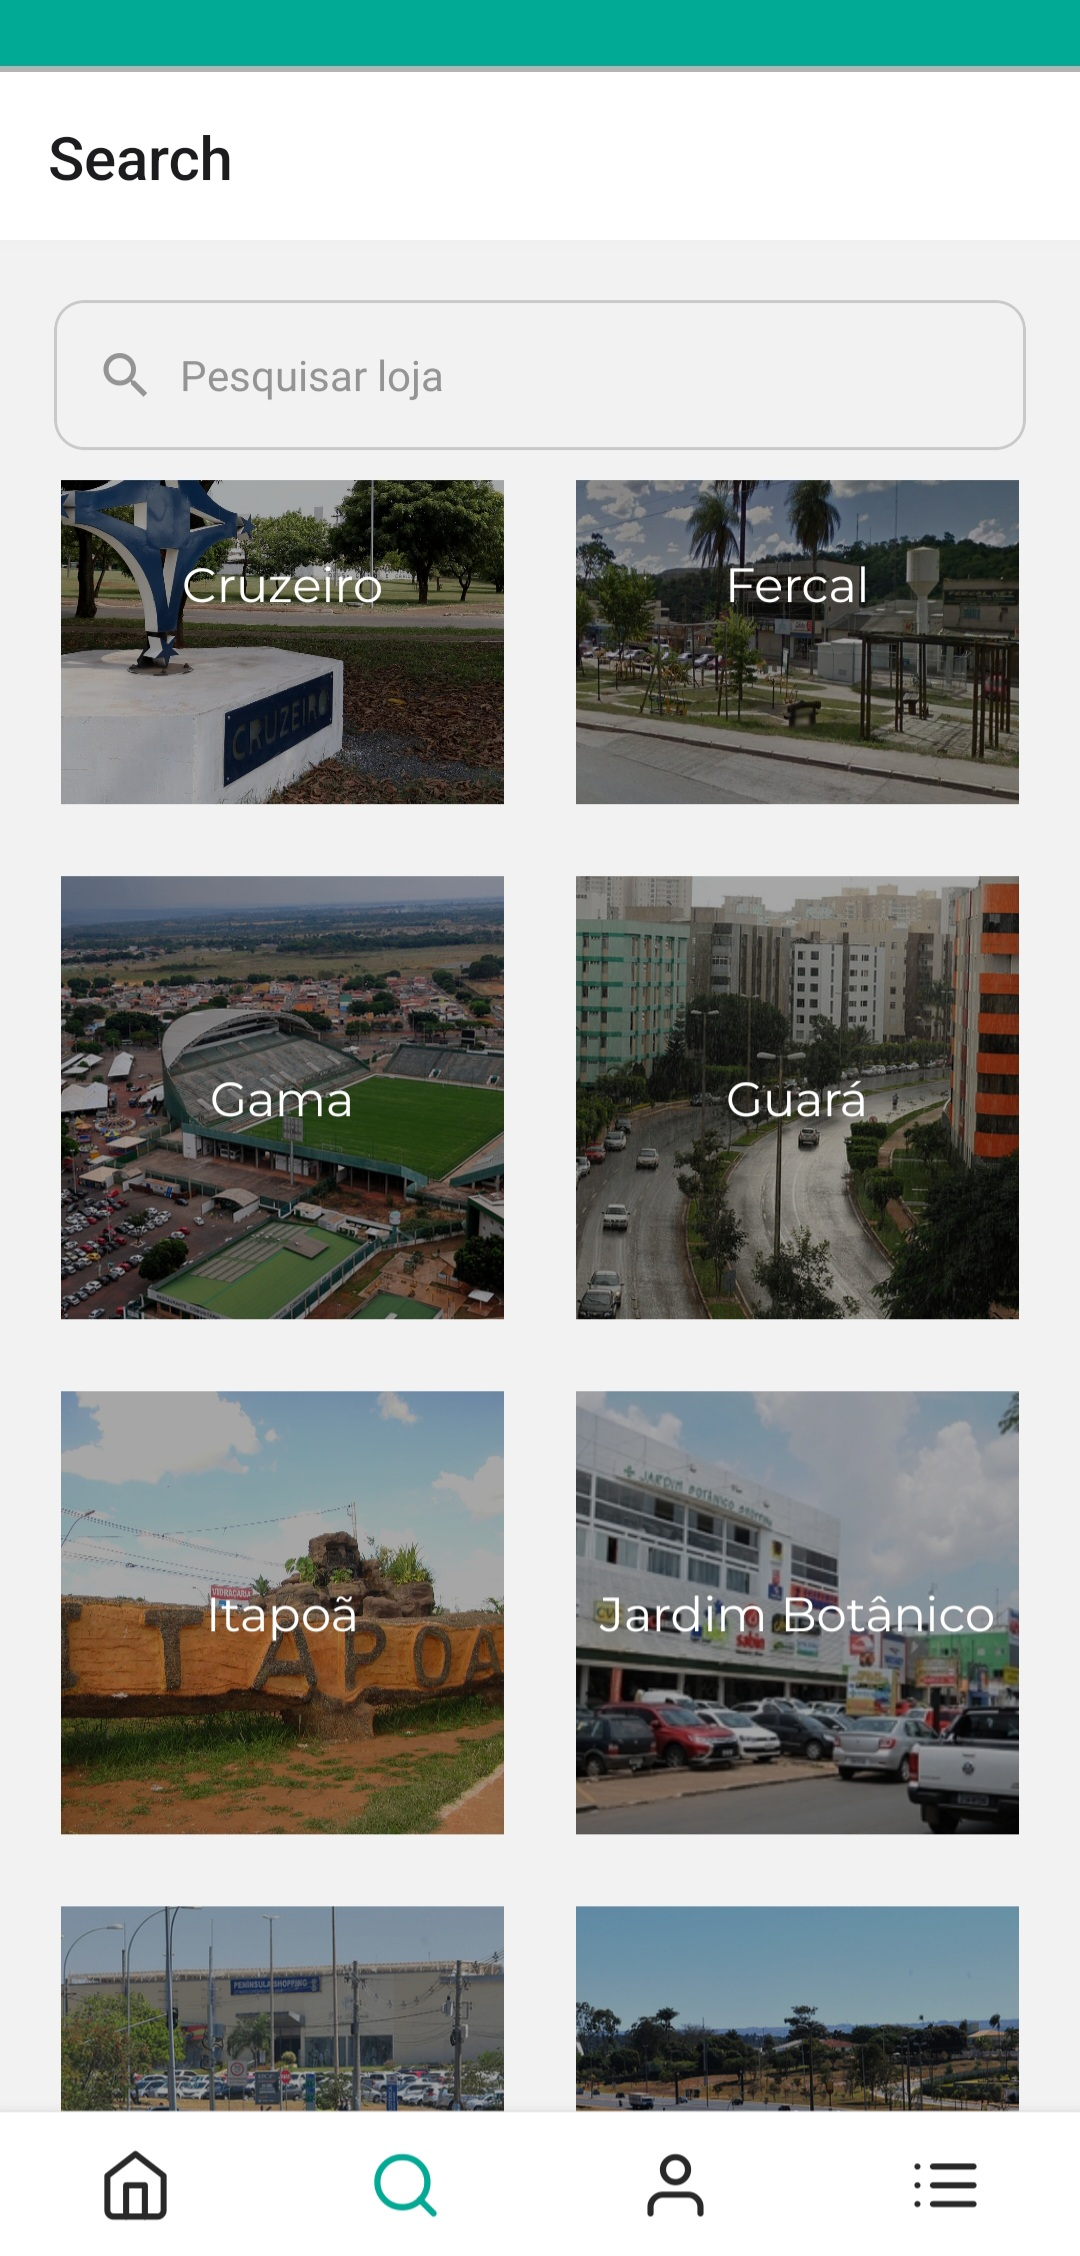
\includegraphics[keepaspectratio=true,scale=0.16]{figuras/filtro_loja_regiao.jpg}
	\caption{Tela de pesquisa de lojas por região administrativa}
        \label{tela-pesquisa-loja-regiao-app}
\end{figure}

\subsection{Adicionar e Editar Endereço}
Na tela de configurações existe a opção de endereço, como mostra a Figura \ref{tela-config-app}. Ao clicar nesta opção, o Aplicativo irá redirecionar para a tela de cadastro e edição de endereço, onde é possível adicionar ou alterar o endereço vinculado ao seu perfil de usuário nesta CSA, como é possível ver na Figura \ref{tela-endereco-app}.

\begin{figure}[h]
	\centering
	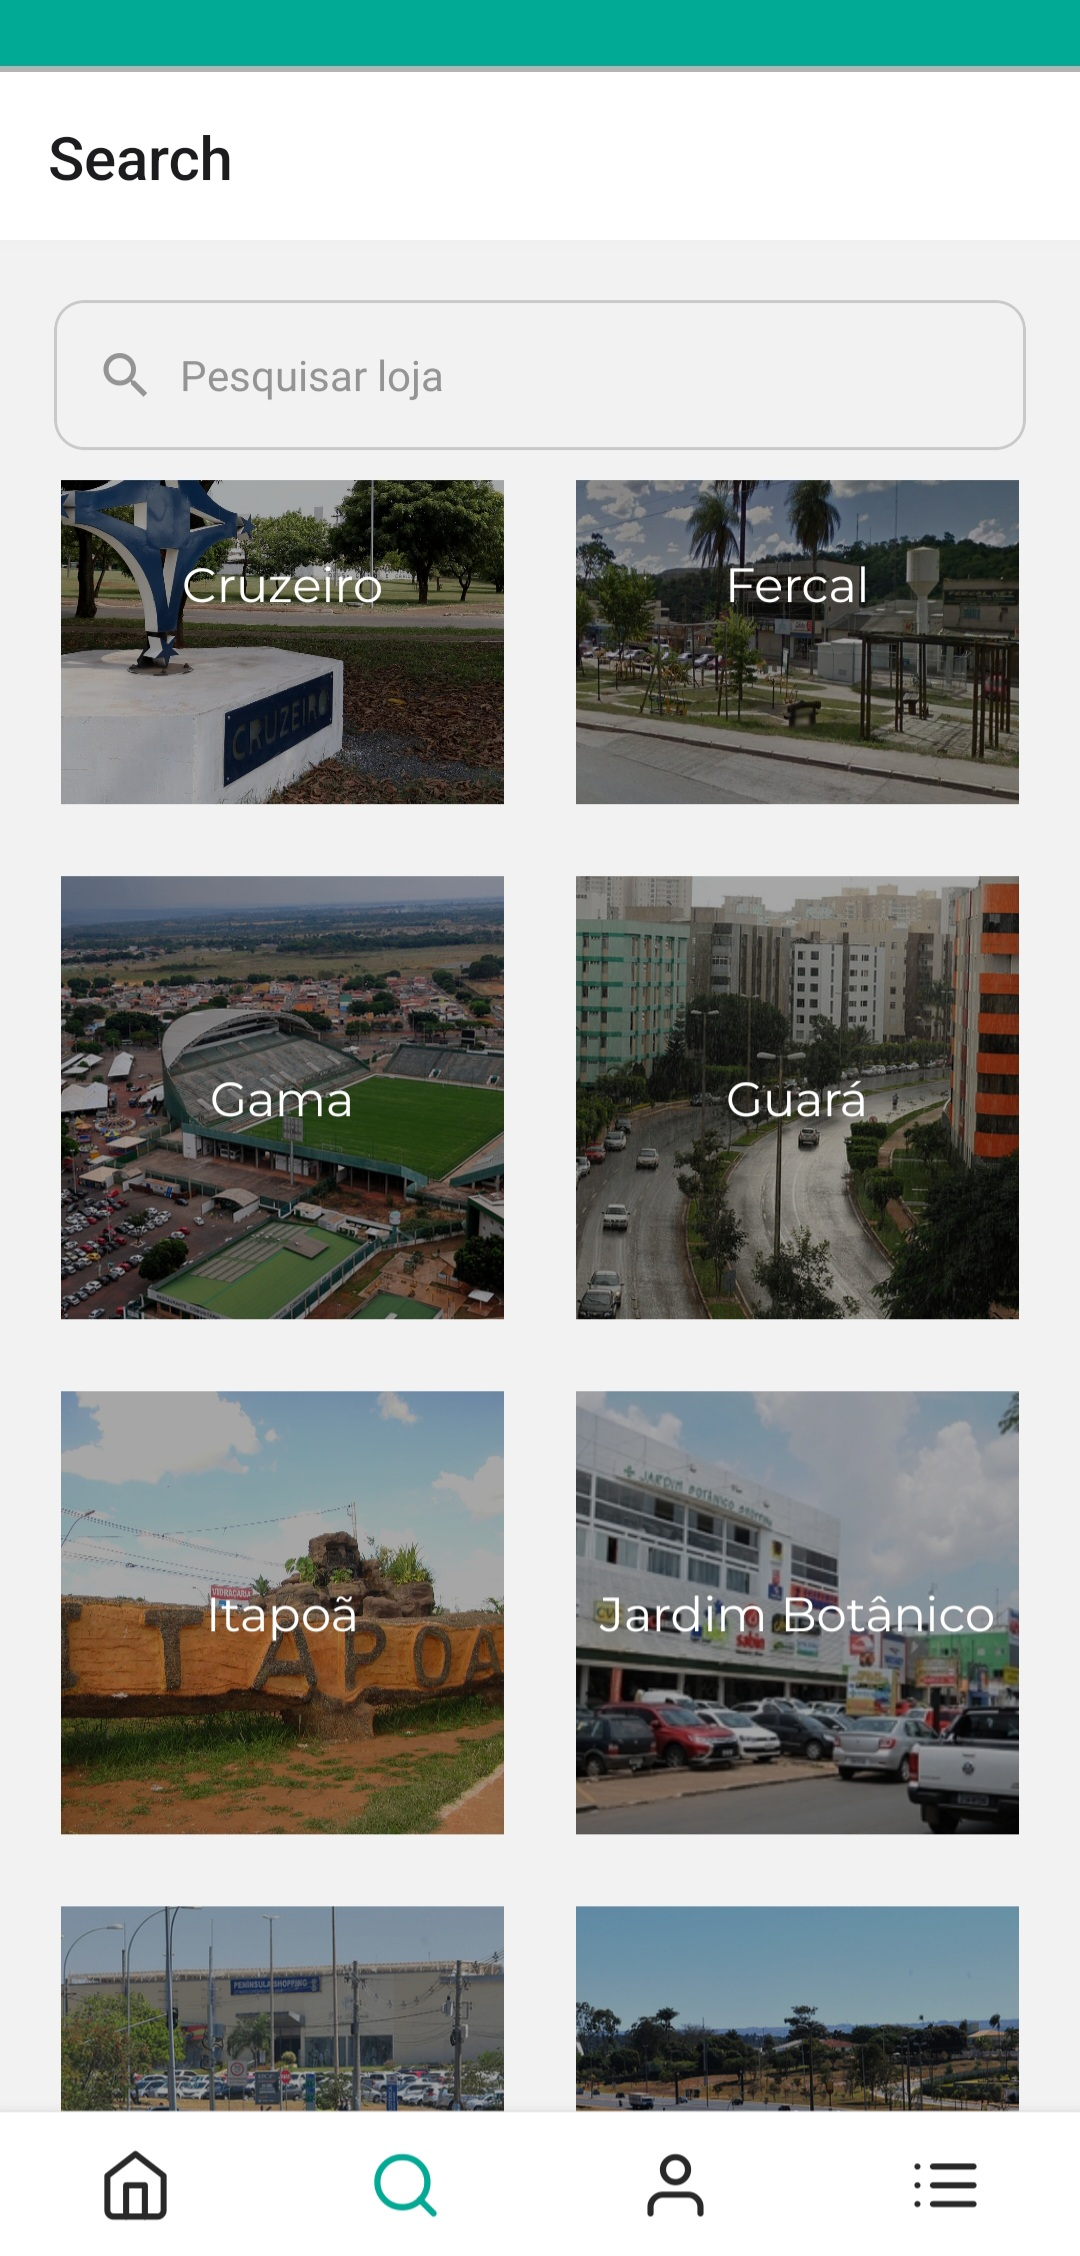
\includegraphics[keepaspectratio=true,scale=0.16]{figuras/filtro_loja_regiao.jpg}
	\caption{Tela de pesquisa de configurações}
        \label{tela-config-app}
\end{figure}

\begin{figure}[h]
	\centering
	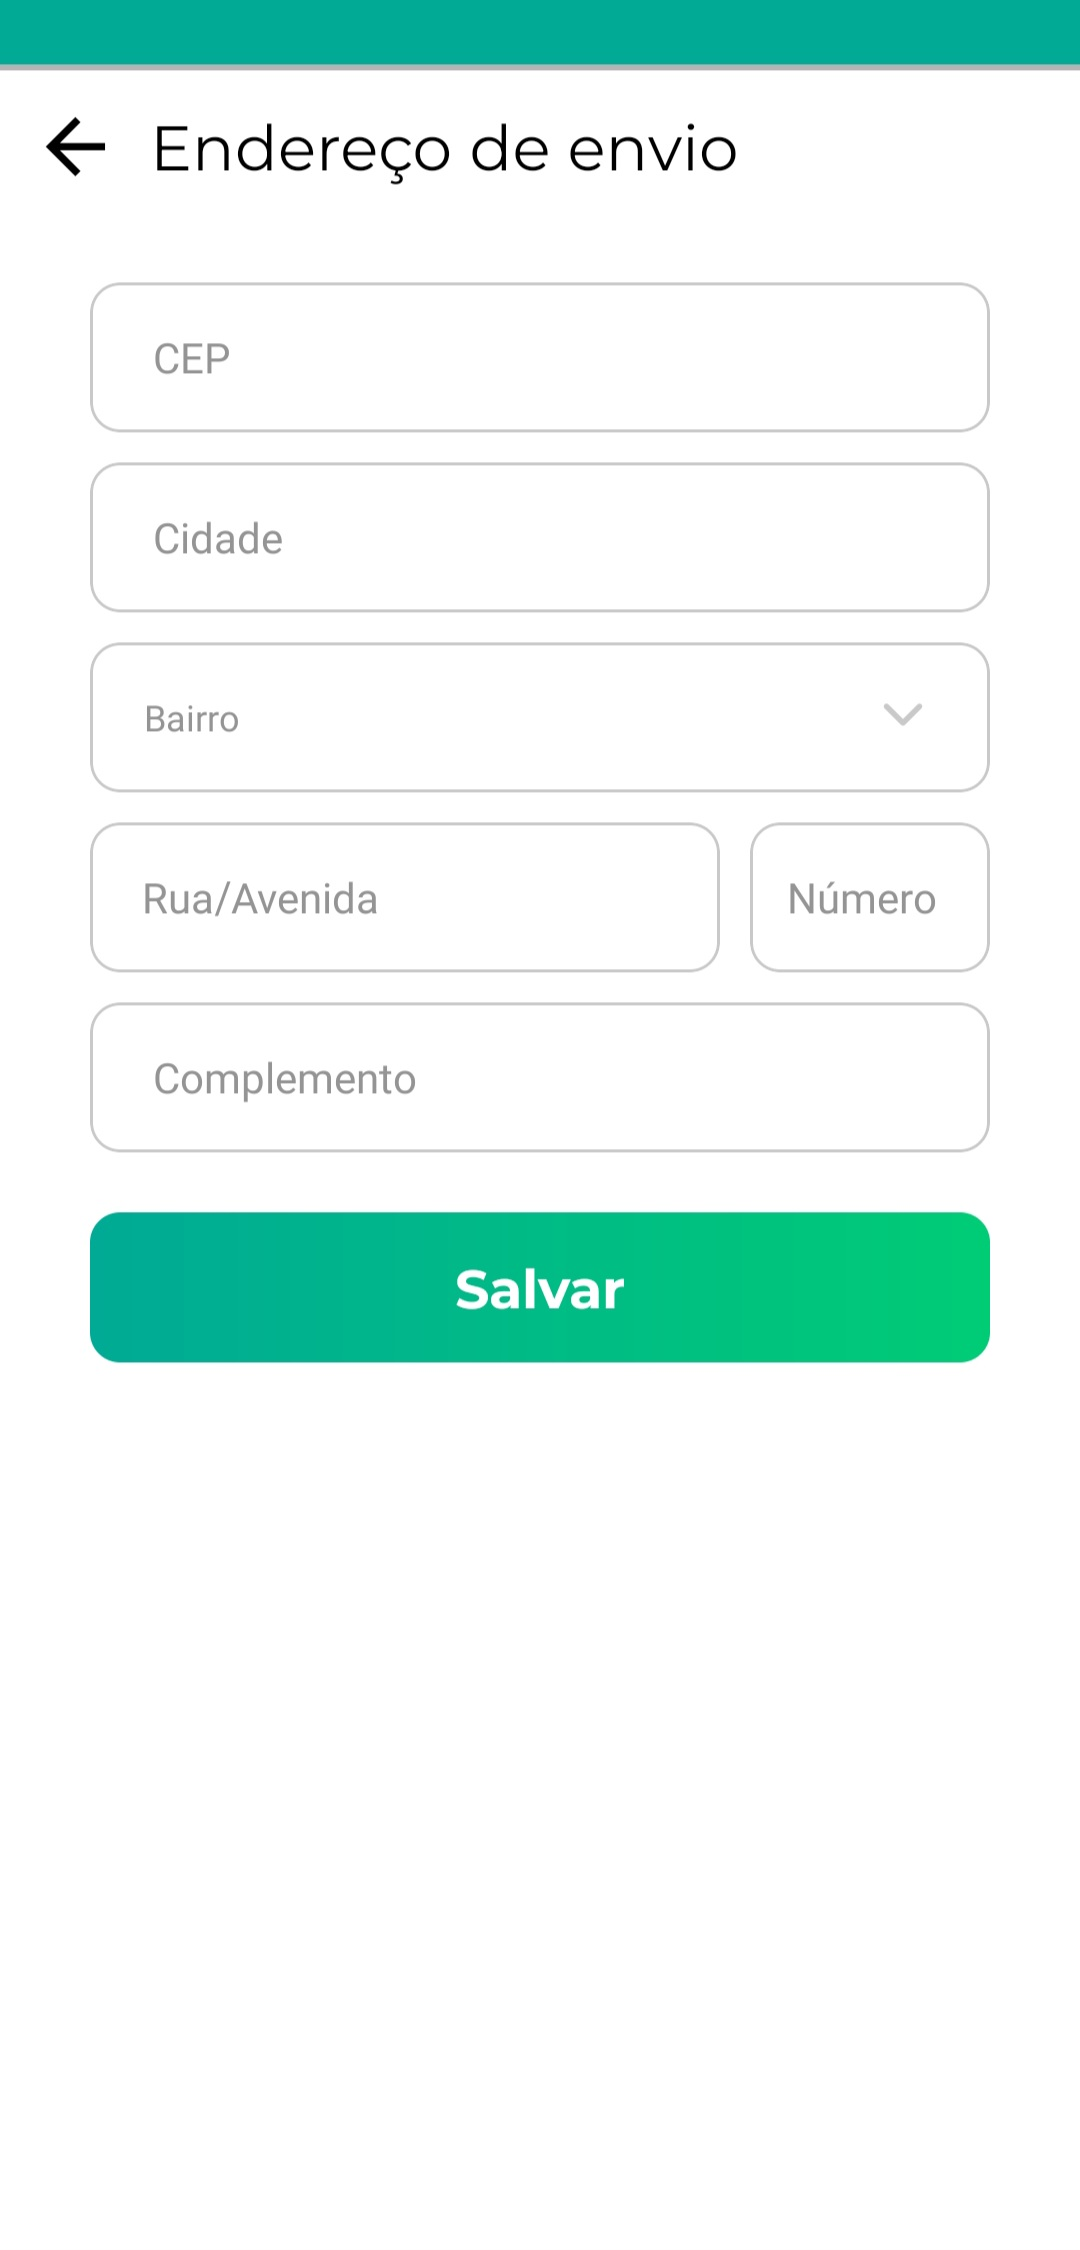
\includegraphics[keepaspectratio=true,scale=0.16]{figuras/tela_endereco.jpg}
	\caption{Tela de endereço}
        \label{tela-edereco-app}
\end{figure}

\subsection{Editar Perfil}
Na tela de configurações mostrada na Figura \ref{tela-config-app}, existe a opção de edição de perfil, que ao ser selecionada redireciona o usuário para uma tela onde é possível editar seu nome e email, como mostra a Figura \ref{tela-perfil-app}.

\begin{figure}[h]
	\centering
	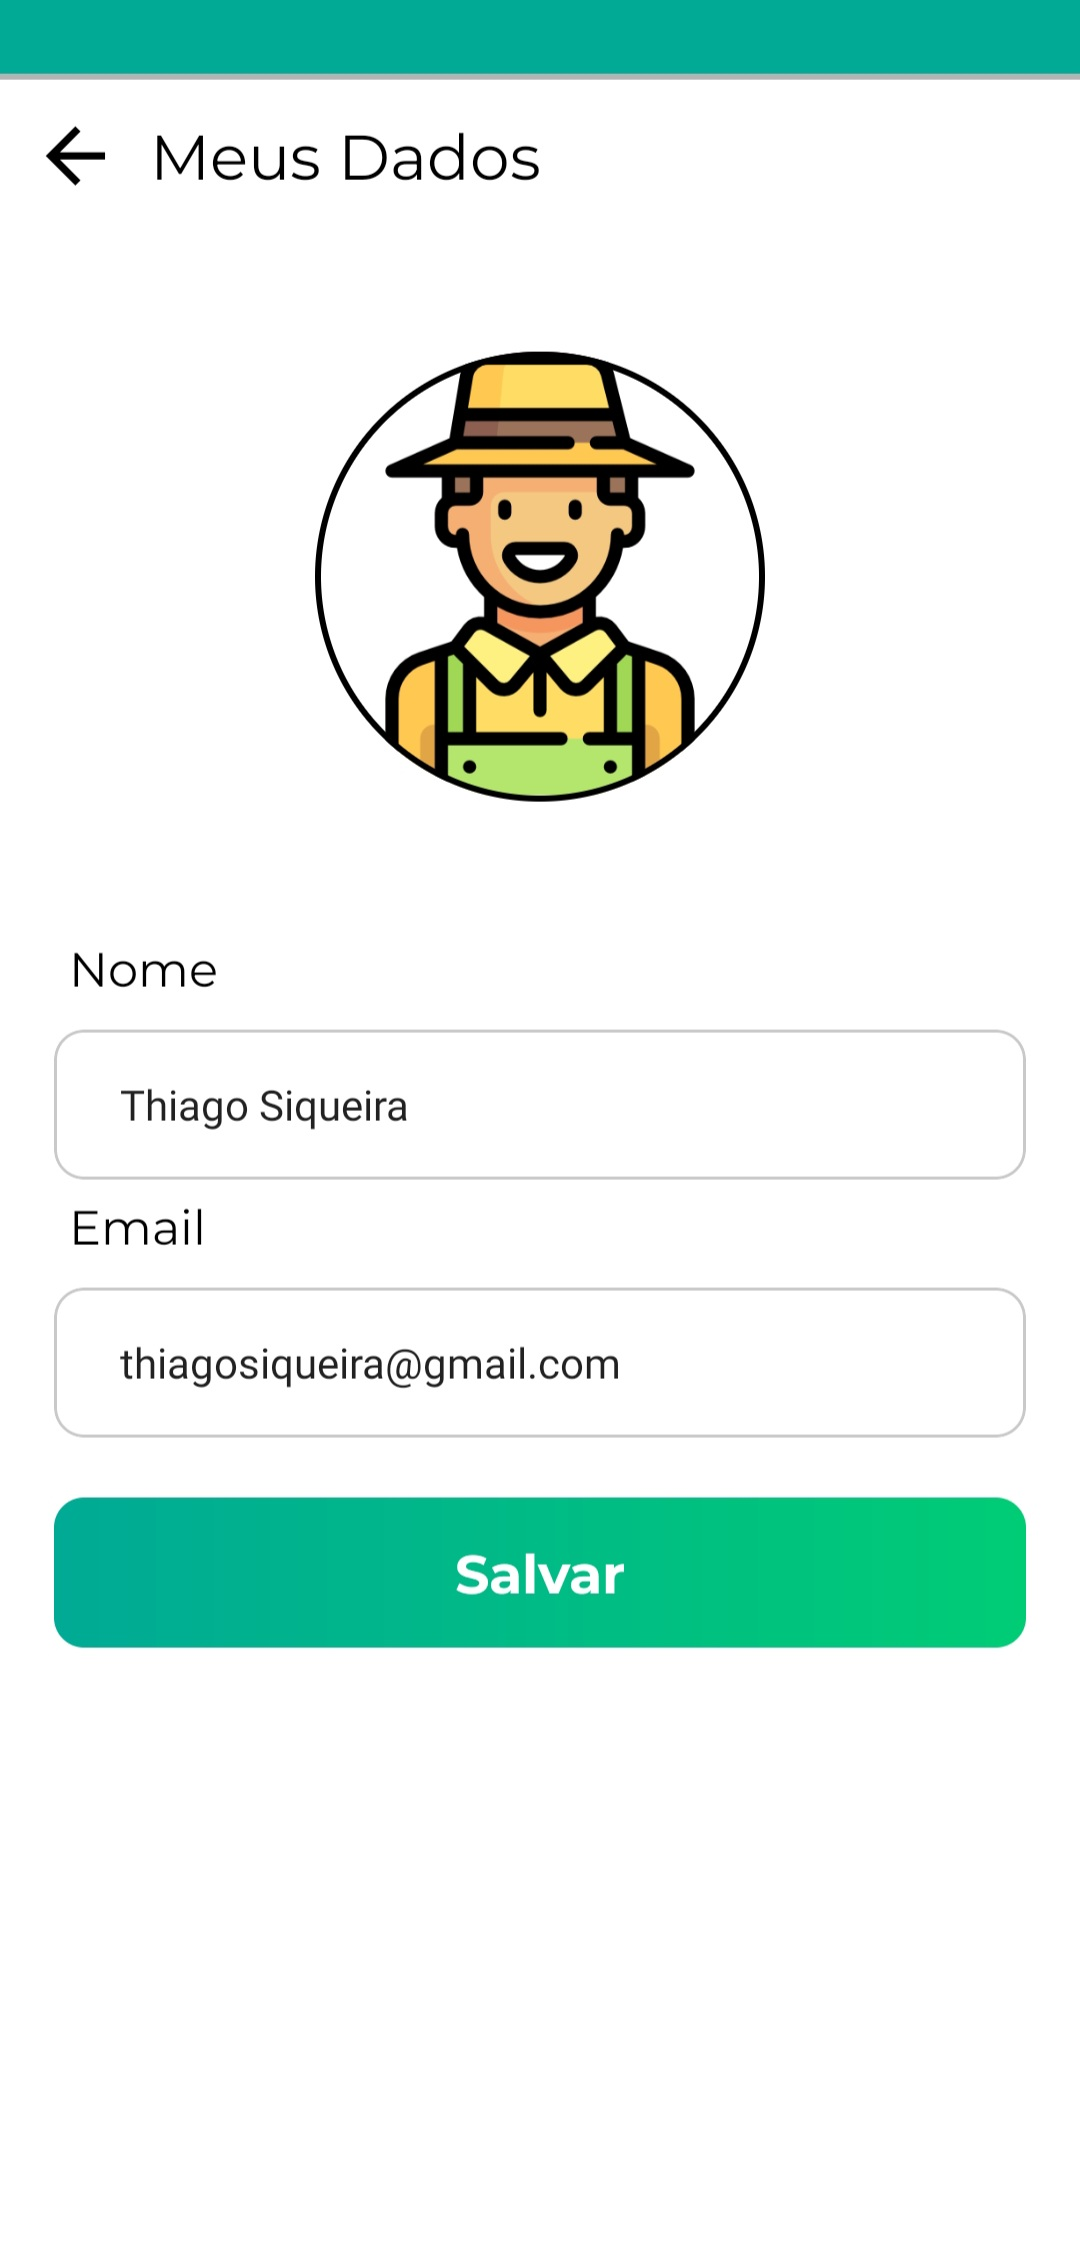
\includegraphics[keepaspectratio=true,scale=0.16]{figuras/tela_perfil.jpg}
	\caption{Tela de perfil}
        \label{tela-perfil-app}
\end{figure}

\subsection{Contatar Dono da Loja}
Dentro da tela principal de uma loja, mostrada na Figura \ref{tela-loja-app}, é possível observar que no canto superior direito existe um ícone do WhatsApp. Clicando neste ícone, o aplicativo irá redirecionar o usuário para o WhatsApp cadastrado pelo dono loja. Esta funcionalidade possibilita uma comunicação direta entre usuário e loja.

\begin{figure}[h]
	\centering
	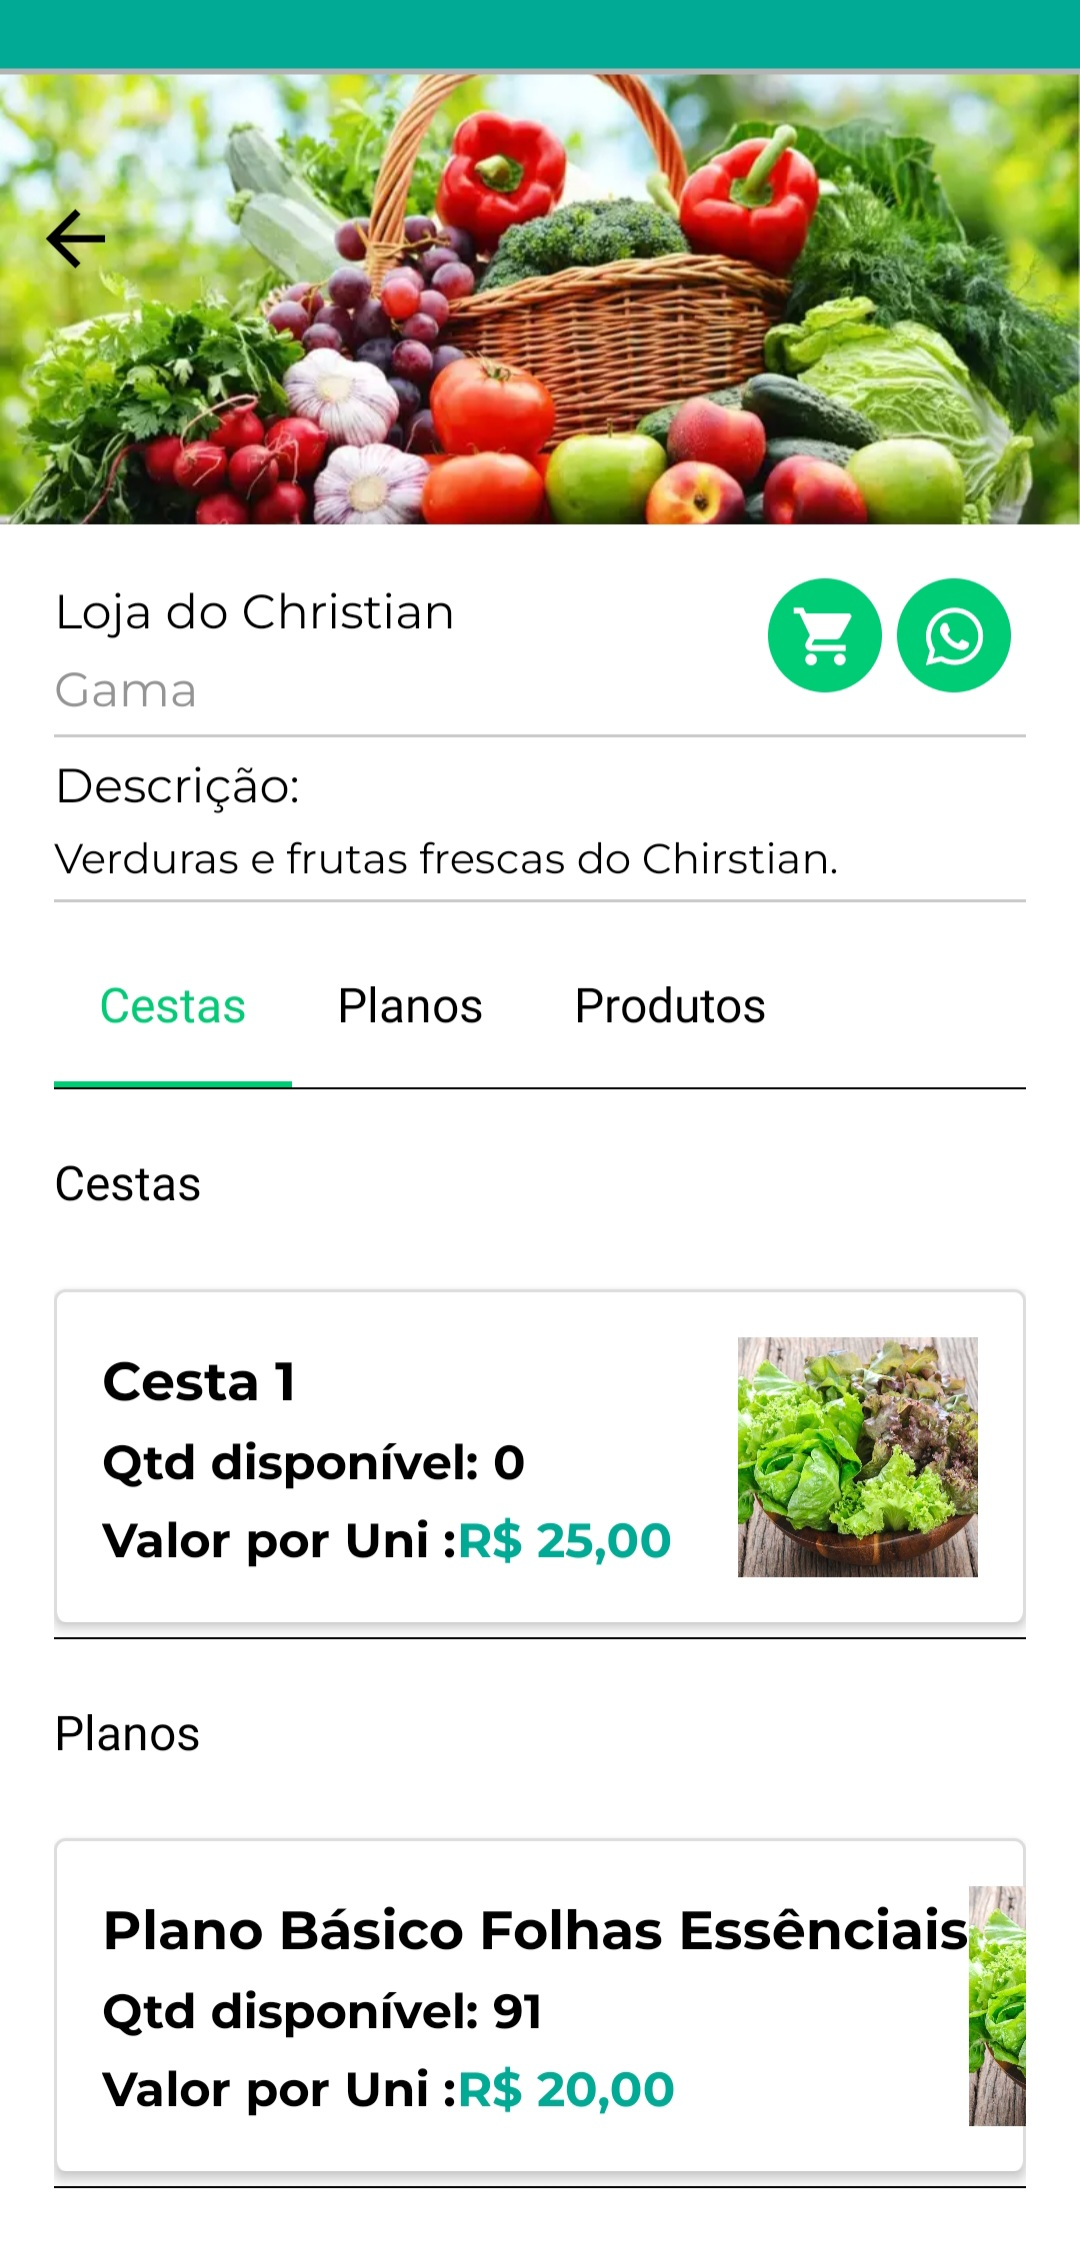
\includegraphics[keepaspectratio=true,scale=0.16]{figuras/tela_loja.jpg}
	\caption{Tela principal de uma loja}
        \label{tela-loja-app}
\end{figure}

\subsection{Visualizar Planos, Cestas e Produtos}
Dentro da tela principal de uma loja, existe uma barra de navegação contendo três categorias: planos, cestas produtos. Selecionando a categoria desejada, é possível visualizar os itens disponíveis, com as quantidades e preços de cada um deles, como mostra a Figura \ref{tela-loja-app}.

\subsection{Realizar Compra}
Ao clicar em um produto, plano ou cesta, é possível escolher a quantidade desejada que deseja e adicionar ao carrinho, como mostra a Figura \ref{tela-adicionar-produto-app}. Ao escolher todos os itens desejados, é possível ir até a tela do seu carrinho, como mostra a Figura \ref{tela-finalizar-compra-app}, e finalizar sua compra. Após finalizar a compra seu pedido será enviado para a loja.

\begin{figure}[h]
	\centering
	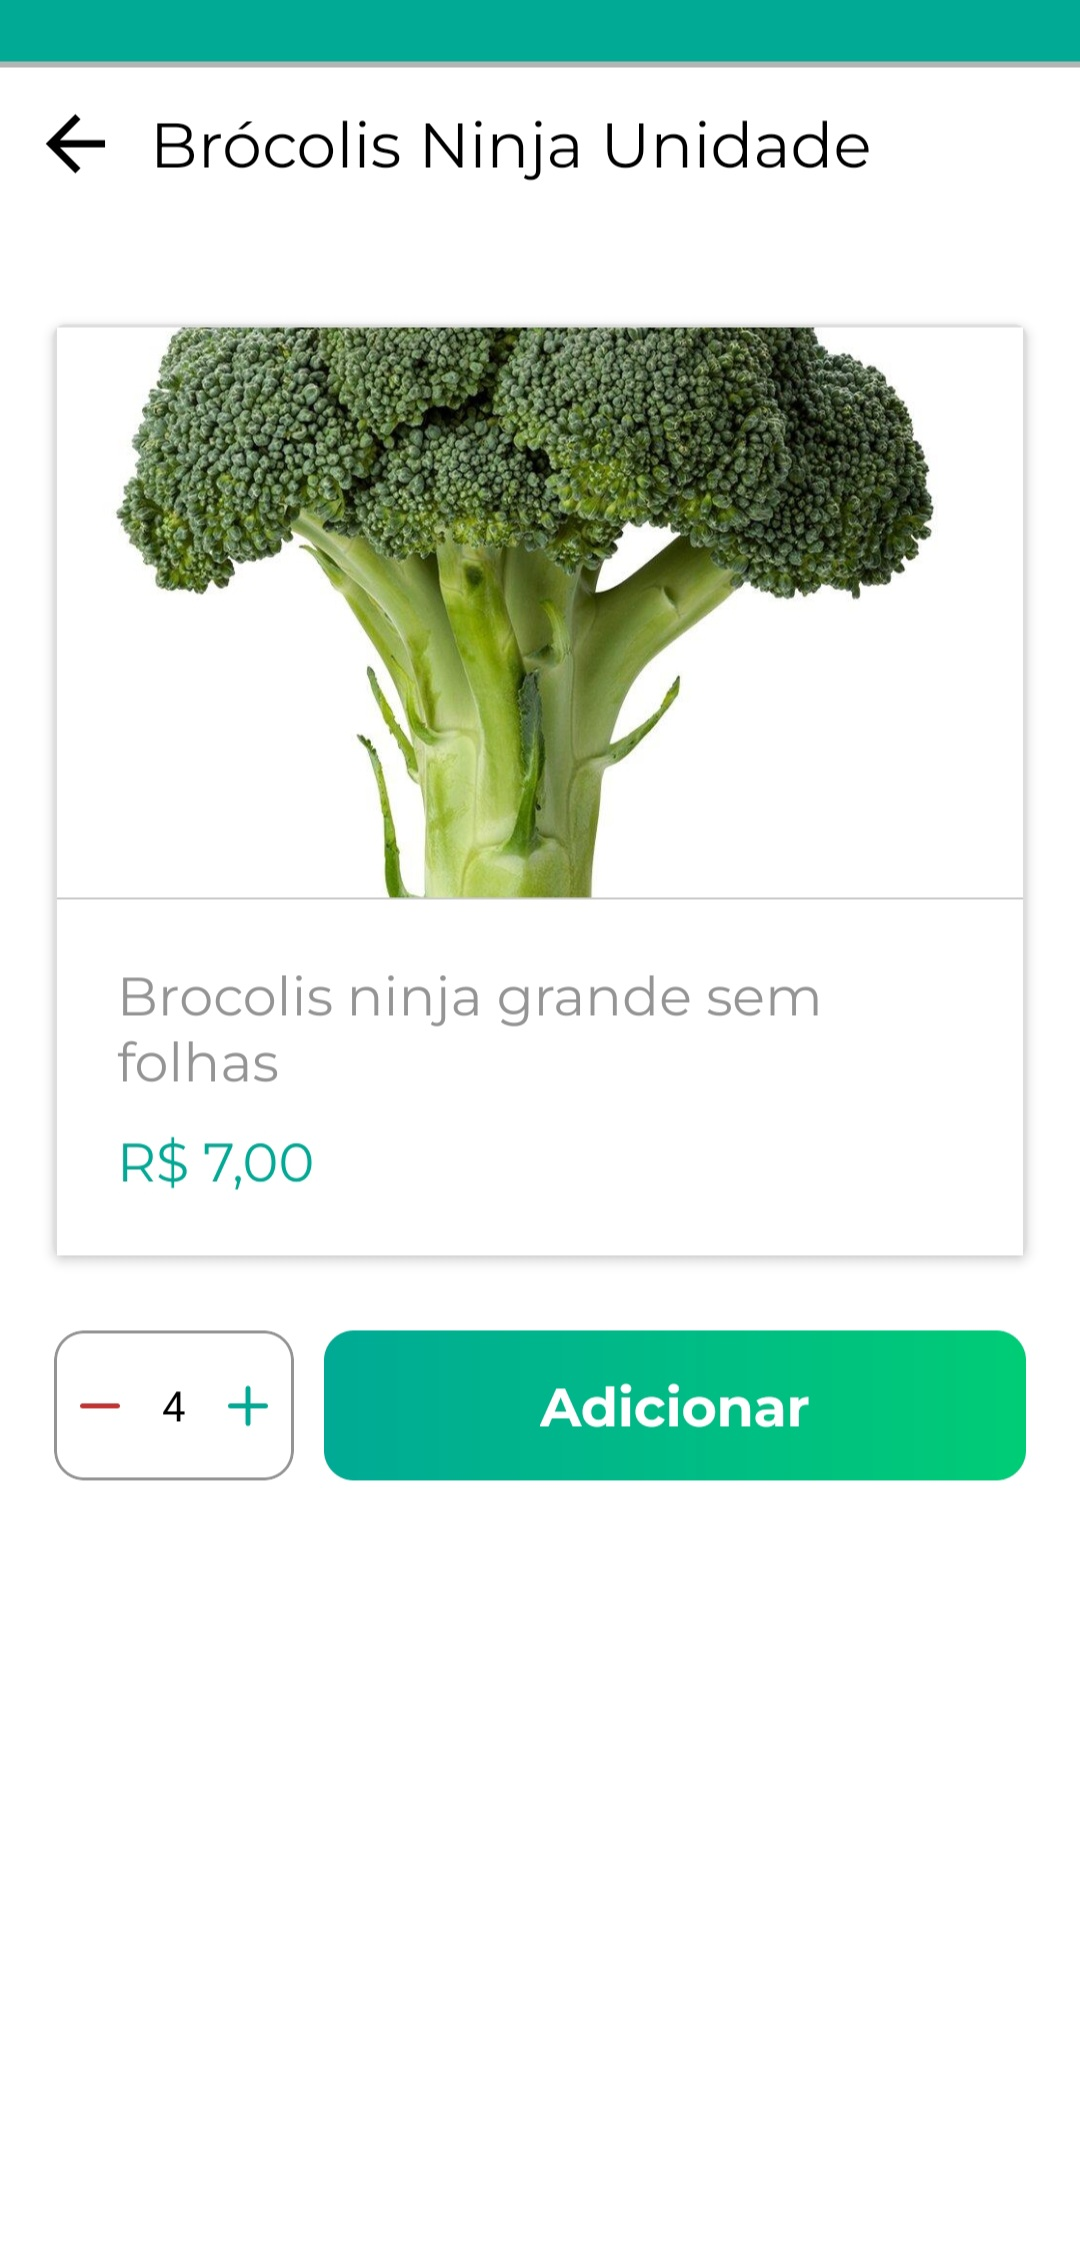
\includegraphics[keepaspectratio=true,scale=0.16]{figuras/adicionar_produto.jpg}
	\caption{Tela de adicionar produto}
        \label{tela-adicionar-produto-app}
\end{figure}

\begin{figure}[h]
	\centering
	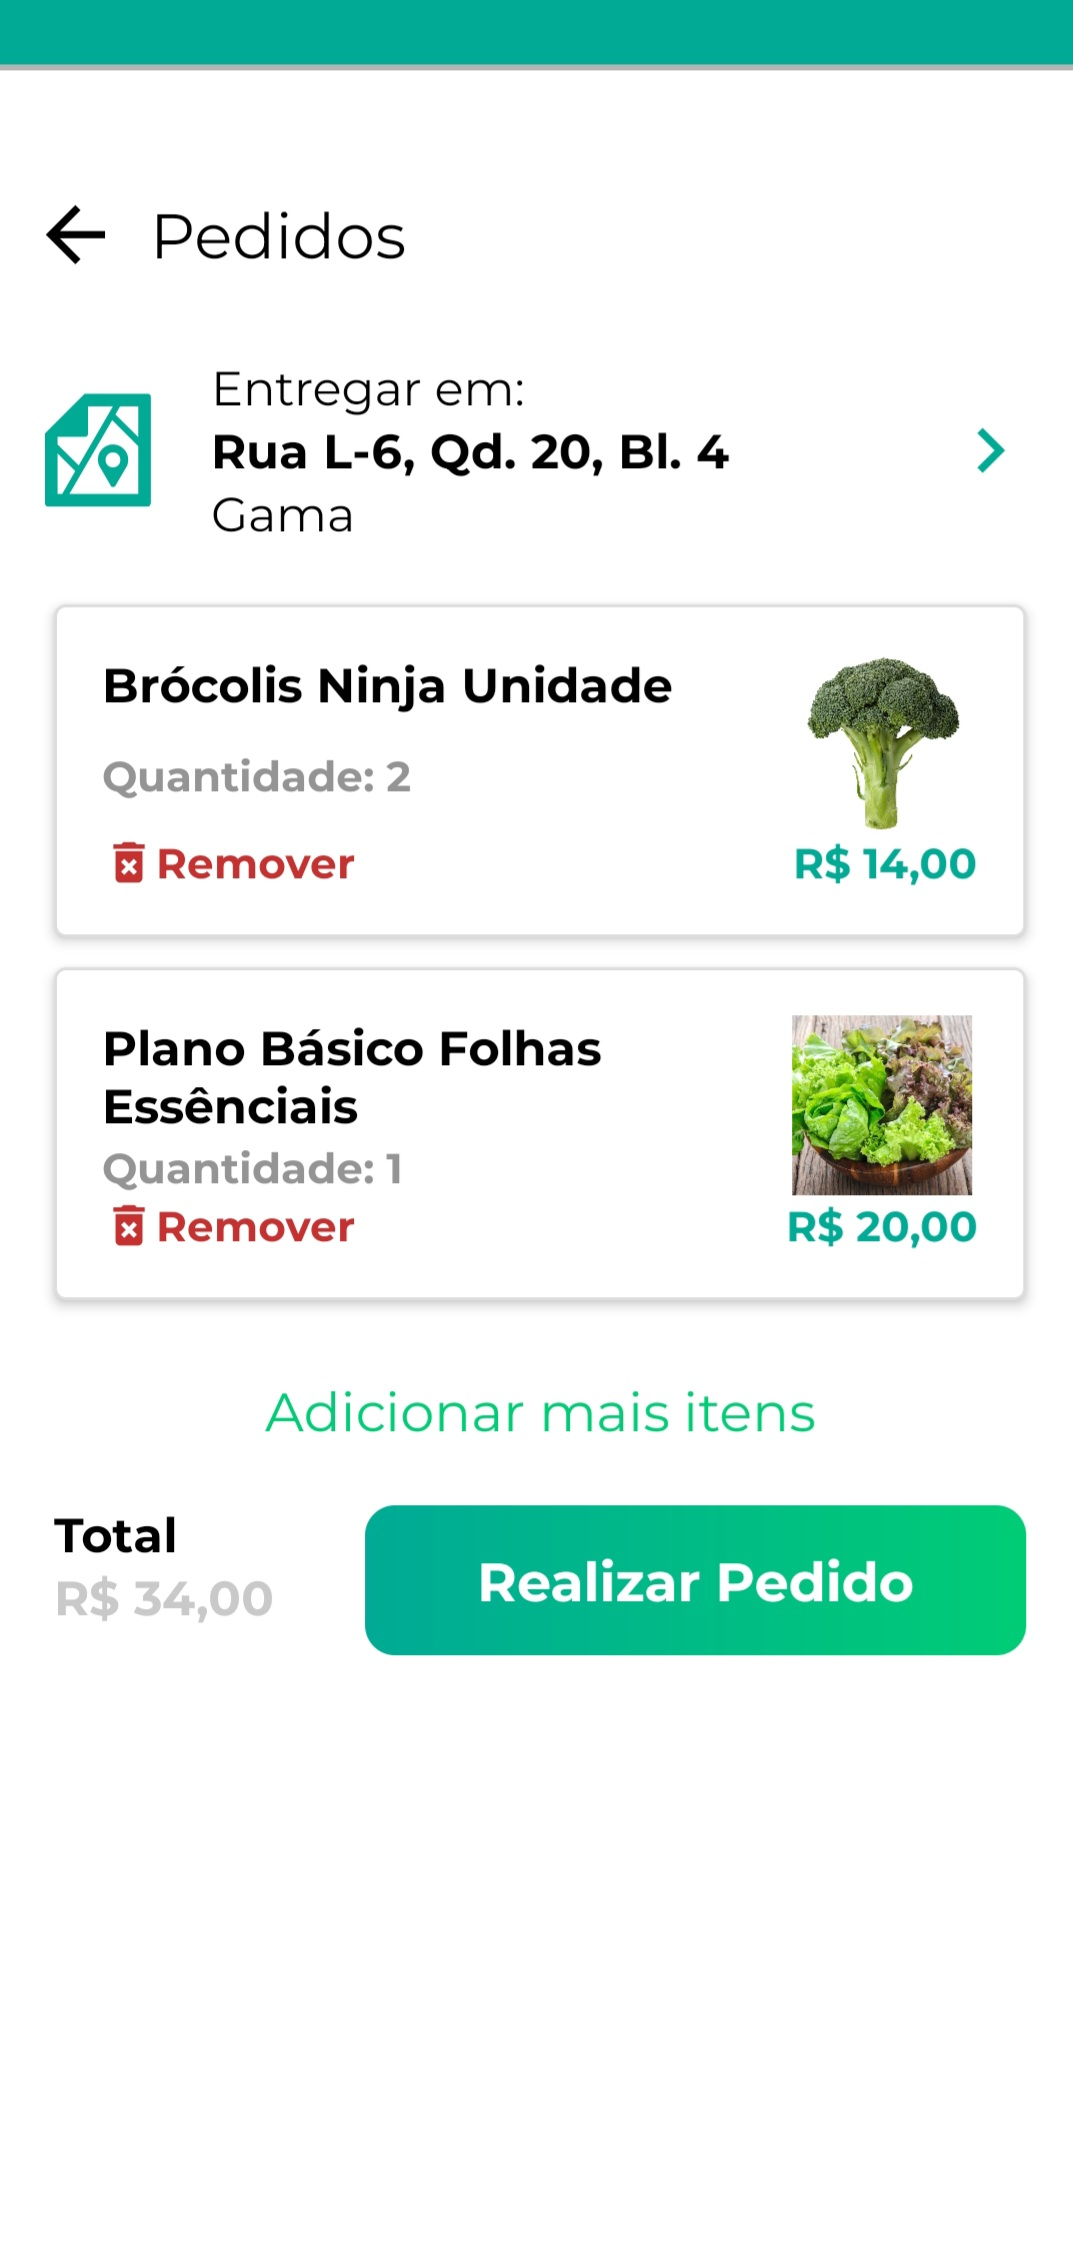
\includegraphics[keepaspectratio=true,scale=0.16]{figuras/finalizar_compra.jpg}
	\caption{Tela de finalizar compra}
        \label{tela-finalizar-compra-app}
\end{figure}

\subsection{Visualizar Histórico de Compras}
Após a realização de uma compra, o usuário será redirecionado para uma tela de histórico, onde é possível ver todas as compras realizadas por ele até o presente momento, como é possível ver na Figura \ref{tela-historico-app}.

\begin{figure}[h]
	\centering
	
\includegraphics[keepaspectratio=true,scale=0.16]{figuras/historico_compras.jpg}
	\caption{Tela histórico de compras}
        \label{tela-historico-app}
\end{figure}

\subsection{Visualizar Planos Assinados e Pular Cesta da Semana}
Na tela de configurações, indicada na Figura \ref{tela-config-app}, é possível selecionar a opção de visualizar os planos assinados. Ao acessar a tela de planos assinados, mostrada na Figura \ref{tela-planos-assinados-app}, é possível visualizar a lista de todos os planos assinados pelo usuário.

Além disso, nesta tela é possível utilizar o campo de "pular cesta semanal", que é um marcador para indicar ao dono da loja que nesta semana o usuário não deseja receber a cesta.

\begin{figure}[h]
	\centering
	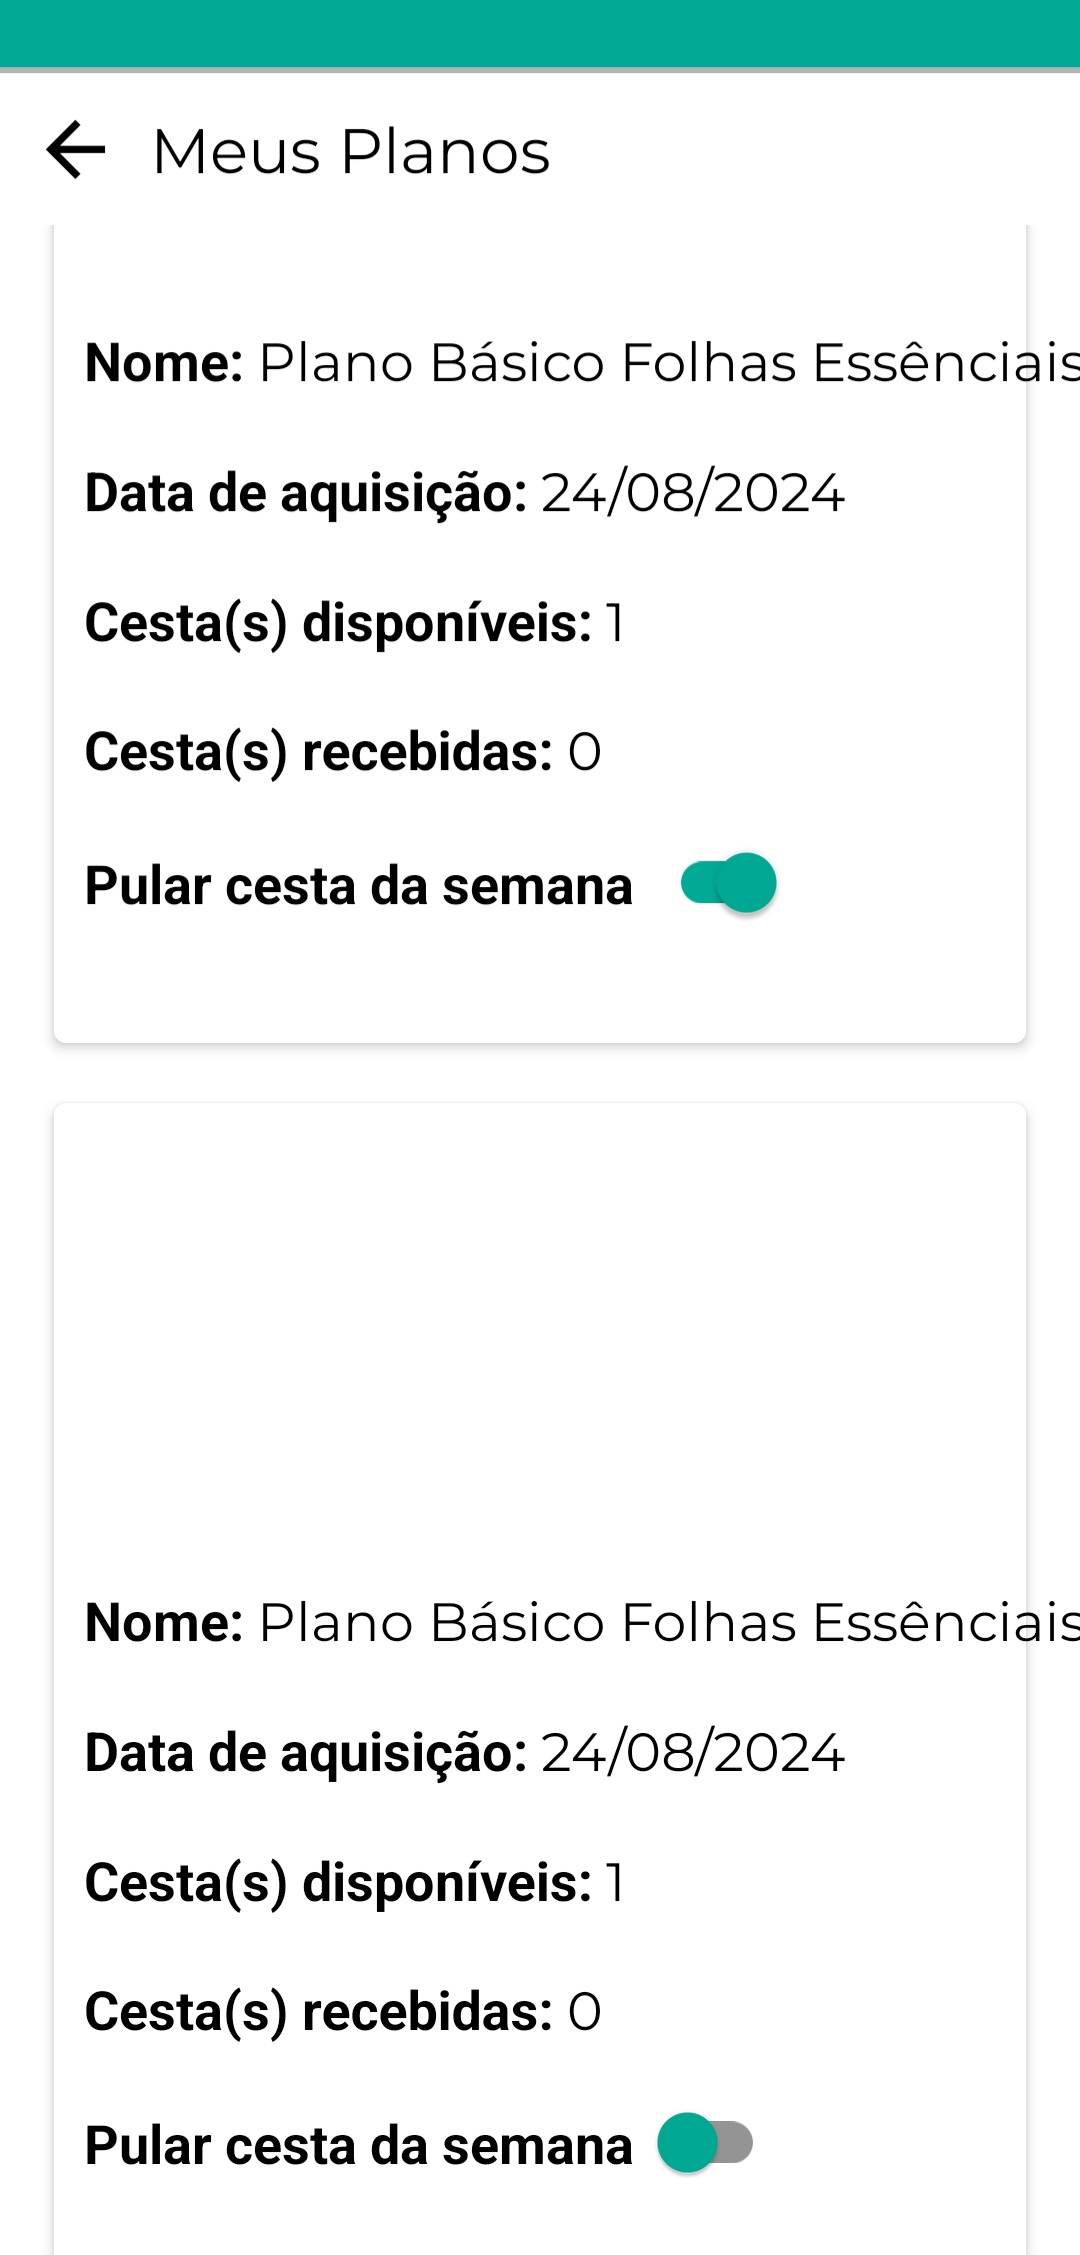
\includegraphics[keepaspectratio=true,scale=0.16]{figuras/planos_assinados.jpg}
	\caption{Tela histórico de compras}
        \label{tela-planos-assinados-app}
\end{figure}